\documentclass{book}
\usepackage[a4paper,top=2.5cm,bottom=2.5cm,left=2.5cm,right=2.5cm]{geometry}
\usepackage{makeidx}
\usepackage{natbib}
\usepackage{graphicx}
\usepackage{multicol}
\usepackage{float}
\usepackage{listings}
\usepackage{color}
\usepackage{ifthen}
\usepackage[table]{xcolor}
\usepackage{textcomp}
\usepackage{alltt}
\usepackage{ifpdf}
\ifpdf
\usepackage[pdftex,
            pagebackref=true,
            colorlinks=true,
            linkcolor=blue,
            unicode
           ]{hyperref}
\else
\usepackage[ps2pdf,
            pagebackref=true,
            colorlinks=true,
            linkcolor=blue,
            unicode
           ]{hyperref}
\usepackage{pspicture}
\fi
\usepackage[utf8]{inputenc}
\usepackage{mathptmx}
\usepackage[scaled=.90]{helvet}
\usepackage{courier}
\usepackage{sectsty}
\usepackage{amssymb}
\usepackage[titles]{tocloft}
\usepackage{doxygen}
\lstset{language=C++,inputencoding=utf8,basicstyle=\footnotesize,breaklines=true,breakatwhitespace=true,tabsize=8,numbers=left }
\makeindex
\setcounter{tocdepth}{3}
\renewcommand{\footrulewidth}{0.4pt}
\renewcommand{\familydefault}{\sfdefault}
\hfuzz=15pt
\setlength{\emergencystretch}{15pt}
\hbadness=750
\tolerance=750
\begin{document}
\hypersetup{pageanchor=false,citecolor=blue}
\begin{titlepage}
\vspace*{7cm}
\begin{center}
{\Large Jenesis \\[1ex]\large 1 }\\
\vspace*{1cm}
{\large Generated by Doxygen 1.8.1.2}\\
\vspace*{0.5cm}
{\small Thu Sep 13 2012 13:06:02}\\
\end{center}
\end{titlepage}
\clearemptydoublepage
\pagenumbering{roman}
\tableofcontents
\clearemptydoublepage
\pagenumbering{arabic}
\hypersetup{pageanchor=true,citecolor=blue}
\chapter{Todo List}
\label{todo}
\hypertarget{todo}{}

\begin{DoxyRefList}
\item[\label{todo__todo000001}%
\hypertarget{todo__todo000001}{}%
Member \hyperlink{classcom_1_1wmbest_1_1jenesis_1_1m68k_1_1instructions_1_1BitwiseInstruction_a79df961b77eeae4ef50ebc9990a3d55c}{com.wmbest.jenesis.m68k.instructions.Bitwise\-Instruction.get\-Instruction} (int value)]M\-O\-V\-E\-P 

B\-T\-S\-T 

B\-C\-H\-G 

B\-C\-L\-R 

B\-S\-E\-T  
\item[\label{todo__todo000006}%
\hypertarget{todo__todo000006}{}%
Member \hyperlink{classcom_1_1wmbest_1_1jenesis_1_1m68k_1_1instructions_1_1ImmediateInstruction_a5ad9ecb37c716bc4d8e877fa9fae76d8}{com.wmbest.jenesis.m68k.instructions.Immediate\-Instruction.get\-Instruction} (int value)]O\-R\-I to C\-C\-R (size 0b00, ea M\-O\-D\-E 0b111) 

O\-R\-I to S\-R (size 0b01, ea M\-O\-D\-E 0b111) 

O\-R\-I 

A\-N\-D\-I to C\-C\-R (size 0b00, ea M\-O\-D\-E 0b111) 

A\-N\-D\-I to S\-R (size 0b01, ea M\-O\-D\-E 0b111) 

A\-N\-D\-I 

E\-O\-R\-I to C\-C\-R (size 0b00, ea M\-O\-D\-E 0b111) 

E\-O\-R\-I to S\-R (size 0b01, ea M\-O\-D\-E 0b111) 

E\-O\-R\-I 

C\-M\-P  
\item[\label{todo__todo000016}%
\hypertarget{todo__todo000016}{}%
Member \hyperlink{classcom_1_1wmbest_1_1jenesis_1_1m68k_1_1instructions_1_1QuickAndBranchInstruction_a926e056f81d08cc66c893fcce53bce6a}{com.wmbest.jenesis.m68k.instructions.Quick\-And\-Branch\-Instruction.get\-Instruction} (int value)]D\-Bcc 

Scc 

B\-R\-A 

B\-S\-R 

Bcc 

M\-O\-V\-E\-Q  
\item[\label{todo__todo000022}%
\hypertarget{todo__todo000022}{}%
Member \hyperlink{classcom_1_1wmbest_1_1jenesis_1_1m68k_1_1instructions_1_1SystemInstruction_a3a02281c96164bd836be2eca75873c07}{com.wmbest.jenesis.m68k.instructions.System\-Instruction.get\-Instruction} (int value)]I\-L\-L\-E\-G\-A\-L 

R\-E\-S\-E\-T 

N\-O\-P 

S\-T\-O\-P 

R\-T\-E 

R\-T\-S 

T\-R\-A\-P\-V 

R\-T\-R 

T\-R\-A\-P 

L\-I\-N\-K (ea M\-O\-D\-E 0b010) 

U\-N\-L\-K (ea M\-O\-D\-E 0b011) 

M\-O\-V\-E U\-S\-P 

M\-O\-V\-E from S\-R (size 0b11) 

N\-E\-G\-X (size 0b00 $\sim$ 0b10) 

M\-O\-V\-E to C\-C\-R (size 0b11) 

N\-E\-G (size 0b00 $\sim$ 0b10) 

M\-O\-V\-E to S\-R (size 0b11) 

N\-O\-T (size 0b00 $\sim$ 0b10) 

E\-X\-T (size 0b10 $\sim$ 0b11, ea M\-O\-D\-E 0b000) 

M\-O\-V\-E\-M (size 0b10 $\sim$ 0b11) 

N\-C\-B\-D (size 0b00) 

S\-W\-A\-P (size 0b01, ea M\-O\-D\-E 0b000) 

P\-E\-A (size 0b01) 

T\-A\-S (size 0b11) 

T\-S\-T (size 0b00 $\sim$ 0b10) 

M\-O\-V\-E\-M (size 0b10 $\sim$ 0b11) 

J\-S\-R (size 0b10) 

J\-M\-P (size 0b11) 
\end{DoxyRefList}
\chapter{Class Index}
\section{Class Hierarchy}
This inheritance list is sorted roughly, but not completely, alphabetically\-:\begin{DoxyCompactList}
\item \contentsline{section}{com.\-wmbest.\-jenesis.\-util.\-Addressable}{\pageref{interfacecom_1_1wmbest_1_1jenesis_1_1util_1_1Addressable}}{}
\begin{DoxyCompactList}
\item \contentsline{section}{com.\-wmbest.\-jenesis.\-rom.\-Rom}{\pageref{classcom_1_1wmbest_1_1jenesis_1_1rom_1_1Rom}}{}
\end{DoxyCompactList}
\item \contentsline{section}{com.\-wmbest.\-jenesis.\-App}{\pageref{classcom_1_1wmbest_1_1jenesis_1_1App}}{}
\item \contentsline{section}{com.\-wmbest.\-jenesis.\-m68k.\-instructions.\-Instruction}{\pageref{classcom_1_1wmbest_1_1jenesis_1_1m68k_1_1instructions_1_1Instruction}}{}
\begin{DoxyCompactList}
\item \contentsline{section}{com.\-wmbest.\-jenesis.\-m68k.\-instructions.\-S\-E\-A\-Instruction}{\pageref{classcom_1_1wmbest_1_1jenesis_1_1m68k_1_1instructions_1_1SEAInstruction}}{}
\begin{DoxyCompactList}
\item \contentsline{section}{com.\-wmbest.\-jenesis.\-m68k.\-instructions.\-Bitwise\-Instruction}{\pageref{classcom_1_1wmbest_1_1jenesis_1_1m68k_1_1instructions_1_1BitwiseInstruction}}{}
\item \contentsline{section}{com.\-wmbest.\-jenesis.\-m68k.\-instructions.\-System\-Instruction}{\pageref{classcom_1_1wmbest_1_1jenesis_1_1m68k_1_1instructions_1_1SystemInstruction}}{}
\item \contentsline{section}{com.\-wmbest.\-jenesis.\-m68k.\-instructions.\-Two\-Op\-Instruction}{\pageref{classcom_1_1wmbest_1_1jenesis_1_1m68k_1_1instructions_1_1TwoOpInstruction}}{}
\begin{DoxyCompactList}
\item \contentsline{section}{com.\-wmbest.\-jenesis.\-m68k.\-instructions.\-Add}{\pageref{classcom_1_1wmbest_1_1jenesis_1_1m68k_1_1instructions_1_1Add}}{}
\item \contentsline{section}{com.\-wmbest.\-jenesis.\-m68k.\-instructions.\-And}{\pageref{classcom_1_1wmbest_1_1jenesis_1_1m68k_1_1instructions_1_1And}}{}
\item \contentsline{section}{com.\-wmbest.\-jenesis.\-m68k.\-instructions.\-Immediate\-Instruction}{\pageref{classcom_1_1wmbest_1_1jenesis_1_1m68k_1_1instructions_1_1ImmediateInstruction}}{}
\begin{DoxyCompactList}
\item \contentsline{section}{com.\-wmbest.\-jenesis.\-m68k.\-instructions.\-Add\-I}{\pageref{classcom_1_1wmbest_1_1jenesis_1_1m68k_1_1instructions_1_1AddI}}{}
\item \contentsline{section}{com.\-wmbest.\-jenesis.\-m68k.\-instructions.\-Sub\-I}{\pageref{classcom_1_1wmbest_1_1jenesis_1_1m68k_1_1instructions_1_1SubI}}{}
\end{DoxyCompactList}
\item \contentsline{section}{com.\-wmbest.\-jenesis.\-m68k.\-instructions.\-Move}{\pageref{classcom_1_1wmbest_1_1jenesis_1_1m68k_1_1instructions_1_1Move}}{}
\item \contentsline{section}{com.\-wmbest.\-jenesis.\-m68k.\-instructions.\-Quick\-And\-Branch\-Instruction}{\pageref{classcom_1_1wmbest_1_1jenesis_1_1m68k_1_1instructions_1_1QuickAndBranchInstruction}}{}
\begin{DoxyCompactList}
\item \contentsline{section}{com.\-wmbest.\-jenesis.\-m68k.\-instructions.\-Add\-Q}{\pageref{classcom_1_1wmbest_1_1jenesis_1_1m68k_1_1instructions_1_1AddQ}}{}
\item \contentsline{section}{com.\-wmbest.\-jenesis.\-m68k.\-instructions.\-Sub\-Q}{\pageref{classcom_1_1wmbest_1_1jenesis_1_1m68k_1_1instructions_1_1SubQ}}{}
\end{DoxyCompactList}
\end{DoxyCompactList}
\end{DoxyCompactList}
\end{DoxyCompactList}
\item \contentsline{section}{com.\-wmbest.\-jenesis.\-Main}{\pageref{classcom_1_1wmbest_1_1jenesis_1_1Main}}{}
\item \contentsline{section}{com.\-wmbest.\-jenesis.\-memory.\-Memory}{\pageref{classcom_1_1wmbest_1_1jenesis_1_1memory_1_1Memory}}{}
\item \contentsline{section}{com.\-wmbest.\-jenesis.\-m68k.\-Operand}{\pageref{classcom_1_1wmbest_1_1jenesis_1_1m68k_1_1Operand}}{}
\item \contentsline{section}{com.\-wmbest.\-jenesis.\-m68k.\-Sixty\-Eight\-K}{\pageref{classcom_1_1wmbest_1_1jenesis_1_1m68k_1_1SixtyEightK}}{}
\end{DoxyCompactList}

\chapter{Class Index}
\section{Class List}
Here are the classes, structs, unions and interfaces with brief descriptions\-:\begin{DoxyCompactList}
\item\contentsline{section}{\hyperlink{classcom_1_1wmbest_1_1jenesis_1_1m68k_1_1instructions_1_1Add}{com.\-wmbest.\-jenesis.\-m68k.\-instructions.\-Add} }{\pageref{classcom_1_1wmbest_1_1jenesis_1_1m68k_1_1instructions_1_1Add}}{}
\item\contentsline{section}{\hyperlink{classcom_1_1wmbest_1_1jenesis_1_1m68k_1_1instructions_1_1AddI}{com.\-wmbest.\-jenesis.\-m68k.\-instructions.\-Add\-I} }{\pageref{classcom_1_1wmbest_1_1jenesis_1_1m68k_1_1instructions_1_1AddI}}{}
\item\contentsline{section}{\hyperlink{classcom_1_1wmbest_1_1jenesis_1_1m68k_1_1instructions_1_1AddQ}{com.\-wmbest.\-jenesis.\-m68k.\-instructions.\-Add\-Q} }{\pageref{classcom_1_1wmbest_1_1jenesis_1_1m68k_1_1instructions_1_1AddQ}}{}
\item\contentsline{section}{\hyperlink{interfacecom_1_1wmbest_1_1jenesis_1_1util_1_1Addressable}{com.\-wmbest.\-jenesis.\-util.\-Addressable} }{\pageref{interfacecom_1_1wmbest_1_1jenesis_1_1util_1_1Addressable}}{}
\item\contentsline{section}{\hyperlink{classcom_1_1wmbest_1_1jenesis_1_1m68k_1_1instructions_1_1And}{com.\-wmbest.\-jenesis.\-m68k.\-instructions.\-And} }{\pageref{classcom_1_1wmbest_1_1jenesis_1_1m68k_1_1instructions_1_1And}}{}
\item\contentsline{section}{\hyperlink{classcom_1_1wmbest_1_1jenesis_1_1App}{com.\-wmbest.\-jenesis.\-App} }{\pageref{classcom_1_1wmbest_1_1jenesis_1_1App}}{}
\item\contentsline{section}{\hyperlink{classcom_1_1wmbest_1_1jenesis_1_1m68k_1_1instructions_1_1BitwiseInstruction}{com.\-wmbest.\-jenesis.\-m68k.\-instructions.\-Bitwise\-Instruction} }{\pageref{classcom_1_1wmbest_1_1jenesis_1_1m68k_1_1instructions_1_1BitwiseInstruction}}{}
\item\contentsline{section}{\hyperlink{classcom_1_1wmbest_1_1jenesis_1_1m68k_1_1instructions_1_1ImmediateInstruction}{com.\-wmbest.\-jenesis.\-m68k.\-instructions.\-Immediate\-Instruction} }{\pageref{classcom_1_1wmbest_1_1jenesis_1_1m68k_1_1instructions_1_1ImmediateInstruction}}{}
\item\contentsline{section}{\hyperlink{classcom_1_1wmbest_1_1jenesis_1_1m68k_1_1instructions_1_1Instruction}{com.\-wmbest.\-jenesis.\-m68k.\-instructions.\-Instruction} }{\pageref{classcom_1_1wmbest_1_1jenesis_1_1m68k_1_1instructions_1_1Instruction}}{}
\item\contentsline{section}{\hyperlink{classcom_1_1wmbest_1_1jenesis_1_1Main}{com.\-wmbest.\-jenesis.\-Main} }{\pageref{classcom_1_1wmbest_1_1jenesis_1_1Main}}{}
\item\contentsline{section}{\hyperlink{classcom_1_1wmbest_1_1jenesis_1_1memory_1_1Memory}{com.\-wmbest.\-jenesis.\-memory.\-Memory} }{\pageref{classcom_1_1wmbest_1_1jenesis_1_1memory_1_1Memory}}{}
\item\contentsline{section}{\hyperlink{classcom_1_1wmbest_1_1jenesis_1_1m68k_1_1instructions_1_1Move}{com.\-wmbest.\-jenesis.\-m68k.\-instructions.\-Move} }{\pageref{classcom_1_1wmbest_1_1jenesis_1_1m68k_1_1instructions_1_1Move}}{}
\item\contentsline{section}{\hyperlink{classcom_1_1wmbest_1_1jenesis_1_1m68k_1_1Operand}{com.\-wmbest.\-jenesis.\-m68k.\-Operand} }{\pageref{classcom_1_1wmbest_1_1jenesis_1_1m68k_1_1Operand}}{}
\item\contentsline{section}{\hyperlink{classcom_1_1wmbest_1_1jenesis_1_1m68k_1_1instructions_1_1QuickAndBranchInstruction}{com.\-wmbest.\-jenesis.\-m68k.\-instructions.\-Quick\-And\-Branch\-Instruction} }{\pageref{classcom_1_1wmbest_1_1jenesis_1_1m68k_1_1instructions_1_1QuickAndBranchInstruction}}{}
\item\contentsline{section}{\hyperlink{classcom_1_1wmbest_1_1jenesis_1_1rom_1_1Rom}{com.\-wmbest.\-jenesis.\-rom.\-Rom} }{\pageref{classcom_1_1wmbest_1_1jenesis_1_1rom_1_1Rom}}{}
\item\contentsline{section}{\hyperlink{classcom_1_1wmbest_1_1jenesis_1_1m68k_1_1instructions_1_1SEAInstruction}{com.\-wmbest.\-jenesis.\-m68k.\-instructions.\-S\-E\-A\-Instruction} }{\pageref{classcom_1_1wmbest_1_1jenesis_1_1m68k_1_1instructions_1_1SEAInstruction}}{}
\item\contentsline{section}{\hyperlink{classcom_1_1wmbest_1_1jenesis_1_1m68k_1_1SixtyEightK}{com.\-wmbest.\-jenesis.\-m68k.\-Sixty\-Eight\-K} }{\pageref{classcom_1_1wmbest_1_1jenesis_1_1m68k_1_1SixtyEightK}}{}
\item\contentsline{section}{\hyperlink{classcom_1_1wmbest_1_1jenesis_1_1m68k_1_1instructions_1_1SubI}{com.\-wmbest.\-jenesis.\-m68k.\-instructions.\-Sub\-I} }{\pageref{classcom_1_1wmbest_1_1jenesis_1_1m68k_1_1instructions_1_1SubI}}{}
\item\contentsline{section}{\hyperlink{classcom_1_1wmbest_1_1jenesis_1_1m68k_1_1instructions_1_1SubQ}{com.\-wmbest.\-jenesis.\-m68k.\-instructions.\-Sub\-Q} }{\pageref{classcom_1_1wmbest_1_1jenesis_1_1m68k_1_1instructions_1_1SubQ}}{}
\item\contentsline{section}{\hyperlink{classcom_1_1wmbest_1_1jenesis_1_1m68k_1_1instructions_1_1SystemInstruction}{com.\-wmbest.\-jenesis.\-m68k.\-instructions.\-System\-Instruction} }{\pageref{classcom_1_1wmbest_1_1jenesis_1_1m68k_1_1instructions_1_1SystemInstruction}}{}
\item\contentsline{section}{\hyperlink{classcom_1_1wmbest_1_1jenesis_1_1m68k_1_1instructions_1_1TwoOpInstruction}{com.\-wmbest.\-jenesis.\-m68k.\-instructions.\-Two\-Op\-Instruction} }{\pageref{classcom_1_1wmbest_1_1jenesis_1_1m68k_1_1instructions_1_1TwoOpInstruction}}{}
\end{DoxyCompactList}

\chapter{Class Documentation}
\hypertarget{classcom_1_1wmbest_1_1jenesis_1_1m68k_1_1instructions_1_1Add}{\section{com.\-wmbest.\-jenesis.\-m68k.\-instructions.\-Add Class Reference}
\label{classcom_1_1wmbest_1_1jenesis_1_1m68k_1_1instructions_1_1Add}\index{com.\-wmbest.\-jenesis.\-m68k.\-instructions.\-Add@{com.\-wmbest.\-jenesis.\-m68k.\-instructions.\-Add}}
}
Inheritance diagram for com.\-wmbest.\-jenesis.\-m68k.\-instructions.\-Add\-:\begin{figure}[H]
\begin{center}
\leavevmode
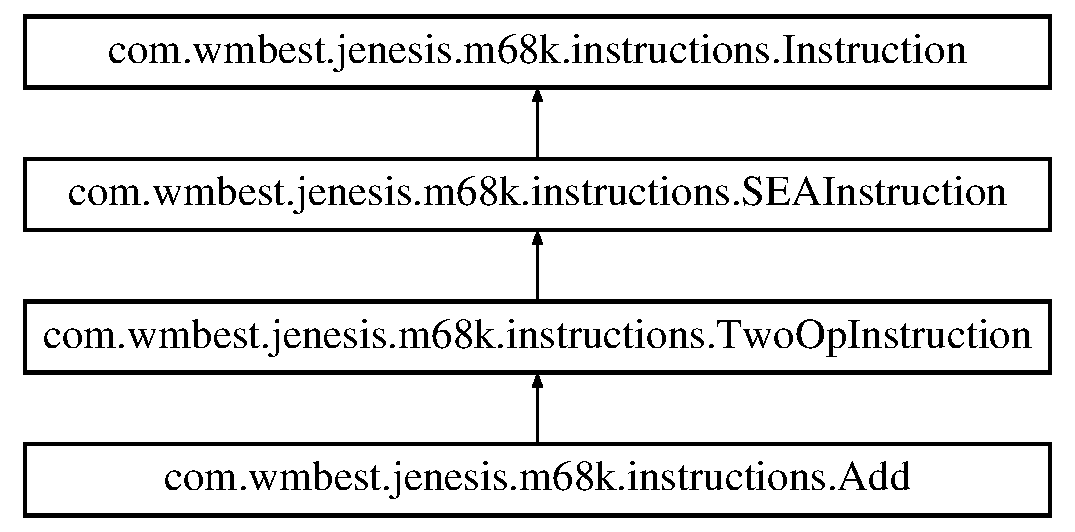
\includegraphics[height=4.000000cm]{classcom_1_1wmbest_1_1jenesis_1_1m68k_1_1instructions_1_1Add}
\end{center}
\end{figure}
\subsection*{Public Member Functions}
\begin{DoxyCompactItemize}
\item 
\hypertarget{classcom_1_1wmbest_1_1jenesis_1_1m68k_1_1instructions_1_1Add_a1b016d95c398cf862696d0d0af9b24bd}{void {\bfseries setup} (int value)}\label{classcom_1_1wmbest_1_1jenesis_1_1m68k_1_1instructions_1_1Add_a1b016d95c398cf862696d0d0af9b24bd}

\item 
\hypertarget{classcom_1_1wmbest_1_1jenesis_1_1m68k_1_1instructions_1_1Add_a4d3d938927508405b8352034e4593a0c}{void {\bfseries handle} ()}\label{classcom_1_1wmbest_1_1jenesis_1_1m68k_1_1instructions_1_1Add_a4d3d938927508405b8352034e4593a0c}

\item 
\hypertarget{classcom_1_1wmbest_1_1jenesis_1_1m68k_1_1instructions_1_1Add_ad5ed3cc71c9e93531446afd43a42717f}{void {\bfseries add\-Dx} (boolean x)}\label{classcom_1_1wmbest_1_1jenesis_1_1m68k_1_1instructions_1_1Add_ad5ed3cc71c9e93531446afd43a42717f}

\item 
\hypertarget{classcom_1_1wmbest_1_1jenesis_1_1m68k_1_1instructions_1_1Add_a56e9f755aea4809196ccdd070ace3768}{void {\bfseries add\-A} ()}\label{classcom_1_1wmbest_1_1jenesis_1_1m68k_1_1instructions_1_1Add_a56e9f755aea4809196ccdd070ace3768}

\item 
\hypertarget{classcom_1_1wmbest_1_1jenesis_1_1m68k_1_1instructions_1_1Add_a56f41c9b847e1c71b46ff831a92843f1}{void {\bfseries add\-E\-A} ()}\label{classcom_1_1wmbest_1_1jenesis_1_1m68k_1_1instructions_1_1Add_a56f41c9b847e1c71b46ff831a92843f1}

\item 
\hypertarget{classcom_1_1wmbest_1_1jenesis_1_1m68k_1_1instructions_1_1Add_af9a31900b69a79370566305c1288e4c8}{void {\bfseries add\-A\-Pre\-With\-X} ()}\label{classcom_1_1wmbest_1_1jenesis_1_1m68k_1_1instructions_1_1Add_af9a31900b69a79370566305c1288e4c8}

\item 
\hypertarget{classcom_1_1wmbest_1_1jenesis_1_1m68k_1_1instructions_1_1Add_ac55226b746c7e44aa407af1e369bebc7}{String {\bfseries disassemble} ()}\label{classcom_1_1wmbest_1_1jenesis_1_1m68k_1_1instructions_1_1Add_ac55226b746c7e44aa407af1e369bebc7}

\end{DoxyCompactItemize}
\subsection*{Additional Inherited Members}


The documentation for this class was generated from the following file\-:\begin{DoxyCompactItemize}
\item 
src/main/java/com/wmbest/jenesis/m68k/instructions/Add.\-java\end{DoxyCompactItemize}

\hypertarget{classcom_1_1wmbest_1_1jenesis_1_1m68k_1_1instructions_1_1AddI}{\section{com.\-wmbest.\-jenesis.\-m68k.\-instructions.\-Add\-I Class Reference}
\label{classcom_1_1wmbest_1_1jenesis_1_1m68k_1_1instructions_1_1AddI}\index{com.\-wmbest.\-jenesis.\-m68k.\-instructions.\-Add\-I@{com.\-wmbest.\-jenesis.\-m68k.\-instructions.\-Add\-I}}
}
Inheritance diagram for com.\-wmbest.\-jenesis.\-m68k.\-instructions.\-Add\-I\-:\begin{figure}[H]
\begin{center}
\leavevmode
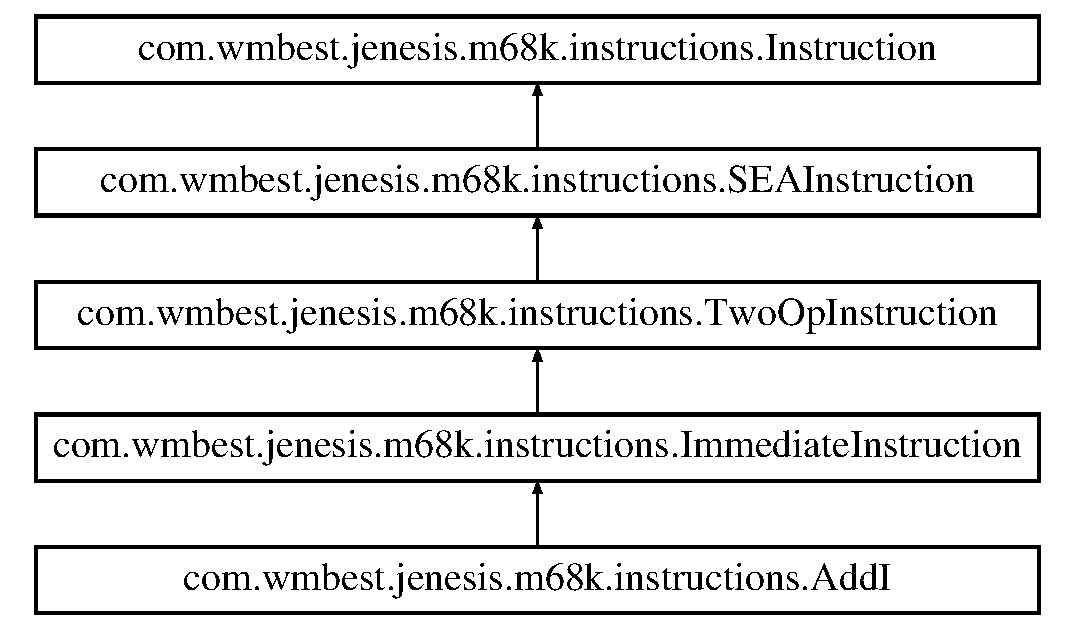
\includegraphics[height=5.000000cm]{classcom_1_1wmbest_1_1jenesis_1_1m68k_1_1instructions_1_1AddI}
\end{center}
\end{figure}
\subsection*{Public Member Functions}
\begin{DoxyCompactItemize}
\item 
\hypertarget{classcom_1_1wmbest_1_1jenesis_1_1m68k_1_1instructions_1_1AddI_afbd2e5dbedea11c1f6625b39e5665b49}{void {\bfseries setup} (int value)}\label{classcom_1_1wmbest_1_1jenesis_1_1m68k_1_1instructions_1_1AddI_afbd2e5dbedea11c1f6625b39e5665b49}

\item 
\hypertarget{classcom_1_1wmbest_1_1jenesis_1_1m68k_1_1instructions_1_1AddI_a5a37a9108e5bb4f8582e1cb6a8d4cb37}{void {\bfseries handle} ()}\label{classcom_1_1wmbest_1_1jenesis_1_1m68k_1_1instructions_1_1AddI_a5a37a9108e5bb4f8582e1cb6a8d4cb37}

\item 
\hypertarget{classcom_1_1wmbest_1_1jenesis_1_1m68k_1_1instructions_1_1AddI_add495e8050021fab4749cb0552a86429}{String {\bfseries disassemble} ()}\label{classcom_1_1wmbest_1_1jenesis_1_1m68k_1_1instructions_1_1AddI_add495e8050021fab4749cb0552a86429}

\end{DoxyCompactItemize}
\subsection*{Additional Inherited Members}


The documentation for this class was generated from the following file\-:\begin{DoxyCompactItemize}
\item 
src/main/java/com/wmbest/jenesis/m68k/instructions/Add\-I.\-java\end{DoxyCompactItemize}

\hypertarget{classcom_1_1wmbest_1_1jenesis_1_1m68k_1_1instructions_1_1AddQ}{\section{com.\-wmbest.\-jenesis.\-m68k.\-instructions.\-Add\-Q Class Reference}
\label{classcom_1_1wmbest_1_1jenesis_1_1m68k_1_1instructions_1_1AddQ}\index{com.\-wmbest.\-jenesis.\-m68k.\-instructions.\-Add\-Q@{com.\-wmbest.\-jenesis.\-m68k.\-instructions.\-Add\-Q}}
}
Inheritance diagram for com.\-wmbest.\-jenesis.\-m68k.\-instructions.\-Add\-Q\-:\begin{figure}[H]
\begin{center}
\leavevmode
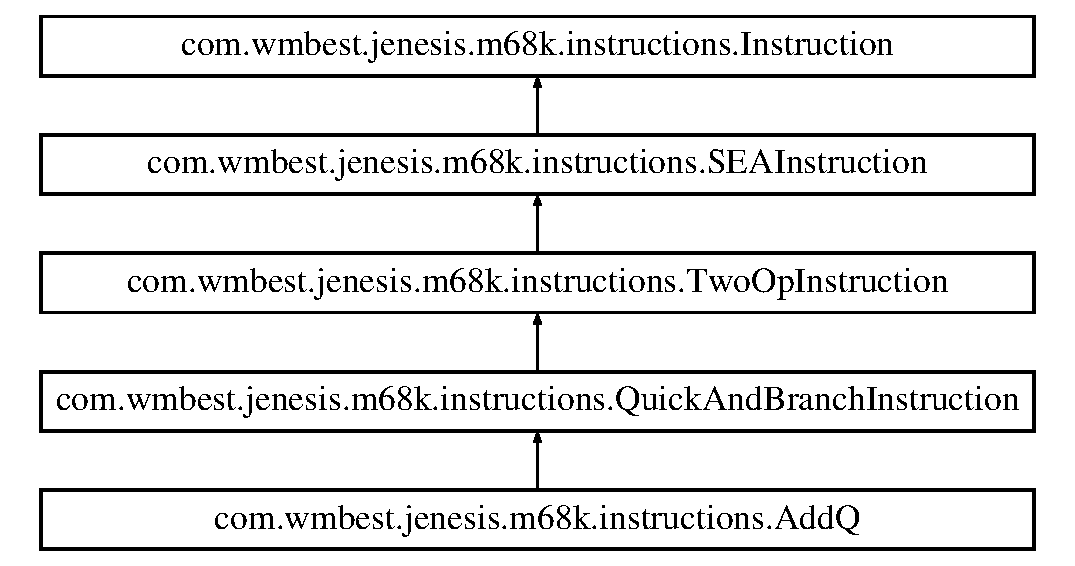
\includegraphics[height=5.000000cm]{classcom_1_1wmbest_1_1jenesis_1_1m68k_1_1instructions_1_1AddQ}
\end{center}
\end{figure}
\subsection*{Public Member Functions}
\begin{DoxyCompactItemize}
\item 
\hypertarget{classcom_1_1wmbest_1_1jenesis_1_1m68k_1_1instructions_1_1AddQ_a6e20b1c7f1fbb28b94fcd653a0c0e03e}{void {\bfseries setup} (int value)}\label{classcom_1_1wmbest_1_1jenesis_1_1m68k_1_1instructions_1_1AddQ_a6e20b1c7f1fbb28b94fcd653a0c0e03e}

\item 
\hypertarget{classcom_1_1wmbest_1_1jenesis_1_1m68k_1_1instructions_1_1AddQ_af29c0fb97d0daaffe7e8754ee6977f1c}{void {\bfseries handle} ()}\label{classcom_1_1wmbest_1_1jenesis_1_1m68k_1_1instructions_1_1AddQ_af29c0fb97d0daaffe7e8754ee6977f1c}

\item 
\hypertarget{classcom_1_1wmbest_1_1jenesis_1_1m68k_1_1instructions_1_1AddQ_a6c438baa32b6d8e80b26f07ab6f07a57}{String {\bfseries disassemble} ()}\label{classcom_1_1wmbest_1_1jenesis_1_1m68k_1_1instructions_1_1AddQ_a6c438baa32b6d8e80b26f07ab6f07a57}

\end{DoxyCompactItemize}
\subsection*{Additional Inherited Members}


The documentation for this class was generated from the following file\-:\begin{DoxyCompactItemize}
\item 
src/main/java/com/wmbest/jenesis/m68k/instructions/Add\-Q.\-java\end{DoxyCompactItemize}

\hypertarget{interfacecom_1_1wmbest_1_1jenesis_1_1util_1_1Addressable}{\section{com.\-wmbest.\-jenesis.\-util.\-Addressable Interface Reference}
\label{interfacecom_1_1wmbest_1_1jenesis_1_1util_1_1Addressable}\index{com.\-wmbest.\-jenesis.\-util.\-Addressable@{com.\-wmbest.\-jenesis.\-util.\-Addressable}}
}
Inheritance diagram for com.\-wmbest.\-jenesis.\-util.\-Addressable\-:\begin{figure}[H]
\begin{center}
\leavevmode
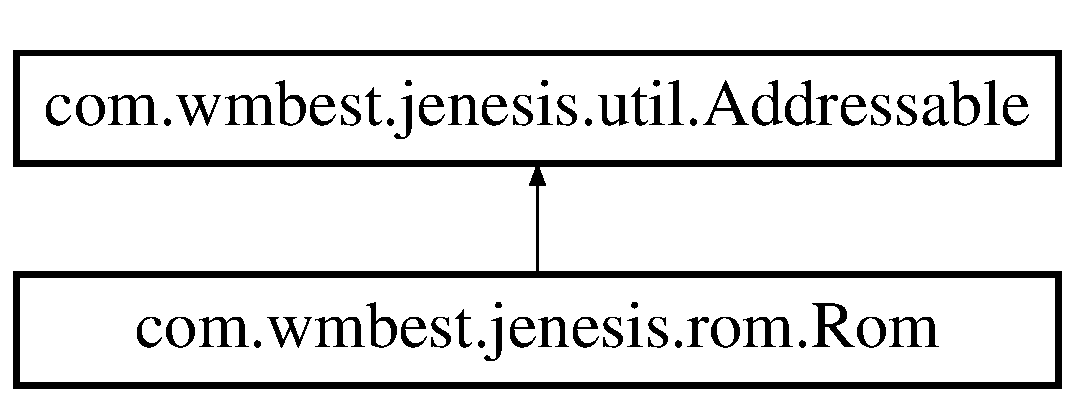
\includegraphics[height=2.000000cm]{interfacecom_1_1wmbest_1_1jenesis_1_1util_1_1Addressable}
\end{center}
\end{figure}
\subsection*{Classes}
\begin{DoxyCompactItemize}
\item 
class {\bfseries Modification\-Exception}
\end{DoxyCompactItemize}
\subsection*{Public Member Functions}
\begin{DoxyCompactItemize}
\item 
\hypertarget{interfacecom_1_1wmbest_1_1jenesis_1_1util_1_1Addressable_a377a40c38f0107f2a1eef13295bc23e4}{int {\bfseries get} (int index)}\label{interfacecom_1_1wmbest_1_1jenesis_1_1util_1_1Addressable_a377a40c38f0107f2a1eef13295bc23e4}

\item 
\hypertarget{interfacecom_1_1wmbest_1_1jenesis_1_1util_1_1Addressable_adf6ae5be6d3c53712f326c5ee1da2b57}{void {\bfseries set} (int index, int value)  throws Modification\-Exception}\label{interfacecom_1_1wmbest_1_1jenesis_1_1util_1_1Addressable_adf6ae5be6d3c53712f326c5ee1da2b57}

\item 
\hypertarget{interfacecom_1_1wmbest_1_1jenesis_1_1util_1_1Addressable_a4e1776d193f1a9b166140ea1b2ecf1e6}{int {\bfseries size} ()}\label{interfacecom_1_1wmbest_1_1jenesis_1_1util_1_1Addressable_a4e1776d193f1a9b166140ea1b2ecf1e6}

\end{DoxyCompactItemize}


The documentation for this interface was generated from the following file\-:\begin{DoxyCompactItemize}
\item 
src/main/java/com/wmbest/jenesis/util/Addressable.\-java\end{DoxyCompactItemize}

\hypertarget{classcom_1_1wmbest_1_1jenesis_1_1m68k_1_1instructions_1_1And}{\section{com.\-wmbest.\-jenesis.\-m68k.\-instructions.\-And Class Reference}
\label{classcom_1_1wmbest_1_1jenesis_1_1m68k_1_1instructions_1_1And}\index{com.\-wmbest.\-jenesis.\-m68k.\-instructions.\-And@{com.\-wmbest.\-jenesis.\-m68k.\-instructions.\-And}}
}
Inheritance diagram for com.\-wmbest.\-jenesis.\-m68k.\-instructions.\-And\-:\begin{figure}[H]
\begin{center}
\leavevmode
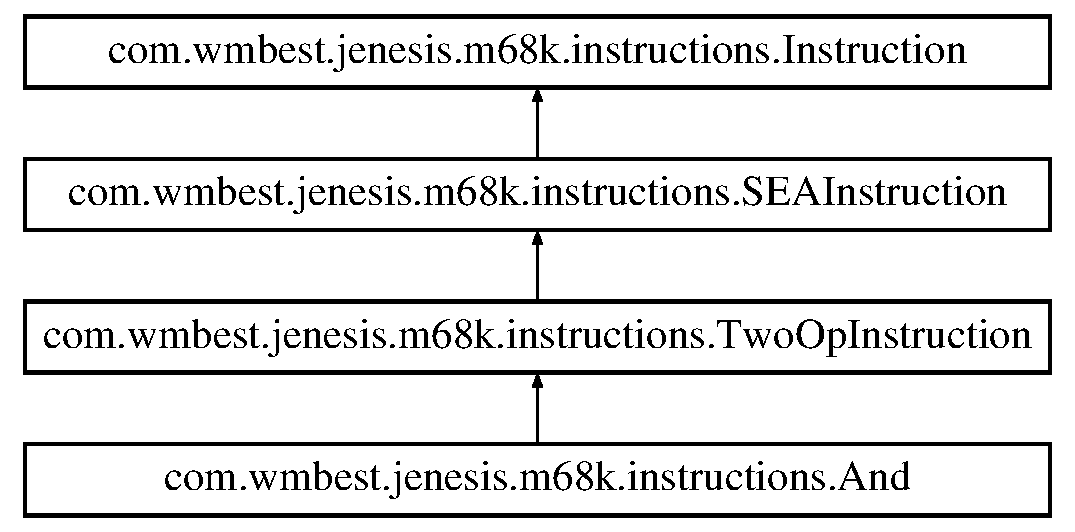
\includegraphics[height=4.000000cm]{classcom_1_1wmbest_1_1jenesis_1_1m68k_1_1instructions_1_1And}
\end{center}
\end{figure}
\subsection*{Public Member Functions}
\begin{DoxyCompactItemize}
\item 
\hypertarget{classcom_1_1wmbest_1_1jenesis_1_1m68k_1_1instructions_1_1And_a07f235df047551864221dd47fc2d9ad7}{void {\bfseries setup} (int value)}\label{classcom_1_1wmbest_1_1jenesis_1_1m68k_1_1instructions_1_1And_a07f235df047551864221dd47fc2d9ad7}

\item 
\hypertarget{classcom_1_1wmbest_1_1jenesis_1_1m68k_1_1instructions_1_1And_aab736f92fc0f72bbb3d21745bd3350dc}{void {\bfseries handle} ()}\label{classcom_1_1wmbest_1_1jenesis_1_1m68k_1_1instructions_1_1And_aab736f92fc0f72bbb3d21745bd3350dc}

\item 
\hypertarget{classcom_1_1wmbest_1_1jenesis_1_1m68k_1_1instructions_1_1And_a6daa43cc0a2cefdfadcfc8b3787f8736}{String {\bfseries disassemble} ()}\label{classcom_1_1wmbest_1_1jenesis_1_1m68k_1_1instructions_1_1And_a6daa43cc0a2cefdfadcfc8b3787f8736}

\end{DoxyCompactItemize}
\subsection*{Additional Inherited Members}


The documentation for this class was generated from the following file\-:\begin{DoxyCompactItemize}
\item 
src/main/java/com/wmbest/jenesis/m68k/instructions/And.\-java\end{DoxyCompactItemize}

\hypertarget{classcom_1_1wmbest_1_1jenesis_1_1App}{\section{com.\-wmbest.\-jenesis.\-App Class Reference}
\label{classcom_1_1wmbest_1_1jenesis_1_1App}\index{com.\-wmbest.\-jenesis.\-App@{com.\-wmbest.\-jenesis.\-App}}
}
\subsection*{Static Public Member Functions}
\begin{DoxyCompactItemize}
\item 
\hypertarget{classcom_1_1wmbest_1_1jenesis_1_1App_a7b524b47846aa794502fb85fe0b7fb1d}{static void {\bfseries main} (String\mbox{[}$\,$\mbox{]} args)}\label{classcom_1_1wmbest_1_1jenesis_1_1App_a7b524b47846aa794502fb85fe0b7fb1d}

\end{DoxyCompactItemize}


\subsection{Detailed Description}
Hello world! 

The documentation for this class was generated from the following file\-:\begin{DoxyCompactItemize}
\item 
src/main/java/com/wmbest/jenesis/App.\-java\end{DoxyCompactItemize}

\hypertarget{classcom_1_1wmbest_1_1jenesis_1_1m68k_1_1instructions_1_1BitwiseInstruction}{\section{com.\-wmbest.\-jenesis.\-m68k.\-instructions.\-Bitwise\-Instruction Class Reference}
\label{classcom_1_1wmbest_1_1jenesis_1_1m68k_1_1instructions_1_1BitwiseInstruction}\index{com.\-wmbest.\-jenesis.\-m68k.\-instructions.\-Bitwise\-Instruction@{com.\-wmbest.\-jenesis.\-m68k.\-instructions.\-Bitwise\-Instruction}}
}
Inheritance diagram for com.\-wmbest.\-jenesis.\-m68k.\-instructions.\-Bitwise\-Instruction\-:\begin{figure}[H]
\begin{center}
\leavevmode
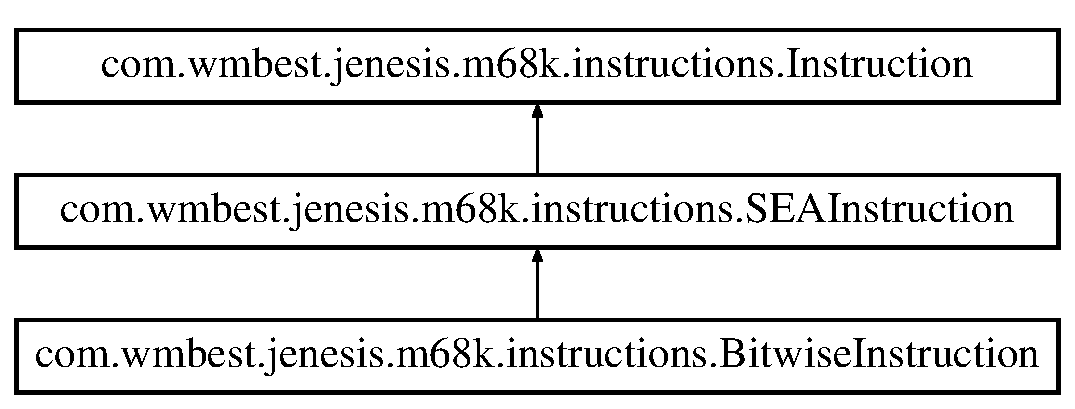
\includegraphics[height=3.000000cm]{classcom_1_1wmbest_1_1jenesis_1_1m68k_1_1instructions_1_1BitwiseInstruction}
\end{center}
\end{figure}
\subsection*{Static Public Member Functions}
\begin{DoxyCompactItemize}
\item 
static \hyperlink{classcom_1_1wmbest_1_1jenesis_1_1m68k_1_1instructions_1_1BitwiseInstruction}{Bitwise\-Instruction} \hyperlink{classcom_1_1wmbest_1_1jenesis_1_1m68k_1_1instructions_1_1BitwiseInstruction_a79df961b77eeae4ef50ebc9990a3d55c}{get\-Instruction} (int value)
\end{DoxyCompactItemize}
\subsection*{Additional Inherited Members}


\subsection{Member Function Documentation}
\hypertarget{classcom_1_1wmbest_1_1jenesis_1_1m68k_1_1instructions_1_1BitwiseInstruction_a79df961b77eeae4ef50ebc9990a3d55c}{\index{com\-::wmbest\-::jenesis\-::m68k\-::instructions\-::\-Bitwise\-Instruction@{com\-::wmbest\-::jenesis\-::m68k\-::instructions\-::\-Bitwise\-Instruction}!get\-Instruction@{get\-Instruction}}
\index{get\-Instruction@{get\-Instruction}!com::wmbest::jenesis::m68k::instructions::BitwiseInstruction@{com\-::wmbest\-::jenesis\-::m68k\-::instructions\-::\-Bitwise\-Instruction}}
\subsubsection[{get\-Instruction}]{\setlength{\rightskip}{0pt plus 5cm}static {\bf Bitwise\-Instruction} com.\-wmbest.\-jenesis.\-m68k.\-instructions.\-Bitwise\-Instruction.\-get\-Instruction (
\begin{DoxyParamCaption}
\item[{int}]{value}
\end{DoxyParamCaption}
)\hspace{0.3cm}{\ttfamily [static]}}}\label{classcom_1_1wmbest_1_1jenesis_1_1m68k_1_1instructions_1_1BitwiseInstruction_a79df961b77eeae4ef50ebc9990a3d55c}
\begin{DoxyRefDesc}{Todo}
\item[\hyperlink{todo__todo000001}{Todo}]M\-O\-V\-E\-P \end{DoxyRefDesc}


\begin{DoxyRefDesc}{Todo}
\item[\hyperlink{todo__todo000002}{Todo}]B\-T\-S\-T \end{DoxyRefDesc}


\begin{DoxyRefDesc}{Todo}
\item[\hyperlink{todo__todo000003}{Todo}]B\-C\-H\-G \end{DoxyRefDesc}


\begin{DoxyRefDesc}{Todo}
\item[\hyperlink{todo__todo000004}{Todo}]B\-C\-L\-R \end{DoxyRefDesc}


\begin{DoxyRefDesc}{Todo}
\item[\hyperlink{todo__todo000005}{Todo}]B\-S\-E\-T \end{DoxyRefDesc}


The documentation for this class was generated from the following file\-:\begin{DoxyCompactItemize}
\item 
src/main/java/com/wmbest/jenesis/m68k/instructions/Bitwise\-Instruction.\-java\end{DoxyCompactItemize}

\hypertarget{classcom_1_1wmbest_1_1jenesis_1_1m68k_1_1instructions_1_1ImmediateInstruction}{\section{com.\-wmbest.\-jenesis.\-m68k.\-instructions.\-Immediate\-Instruction Class Reference}
\label{classcom_1_1wmbest_1_1jenesis_1_1m68k_1_1instructions_1_1ImmediateInstruction}\index{com.\-wmbest.\-jenesis.\-m68k.\-instructions.\-Immediate\-Instruction@{com.\-wmbest.\-jenesis.\-m68k.\-instructions.\-Immediate\-Instruction}}
}
Inheritance diagram for com.\-wmbest.\-jenesis.\-m68k.\-instructions.\-Immediate\-Instruction\-:\begin{figure}[H]
\begin{center}
\leavevmode
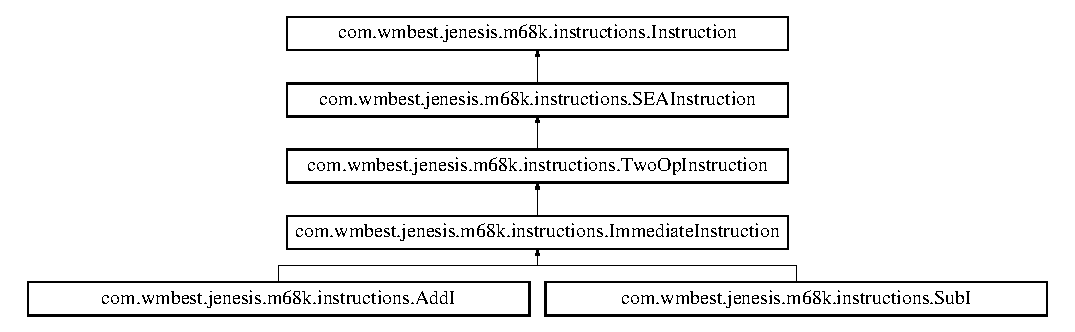
\includegraphics[height=4.011461cm]{classcom_1_1wmbest_1_1jenesis_1_1m68k_1_1instructions_1_1ImmediateInstruction}
\end{center}
\end{figure}
\subsection*{Static Public Member Functions}
\begin{DoxyCompactItemize}
\item 
static \hyperlink{classcom_1_1wmbest_1_1jenesis_1_1m68k_1_1instructions_1_1ImmediateInstruction}{Immediate\-Instruction} \hyperlink{classcom_1_1wmbest_1_1jenesis_1_1m68k_1_1instructions_1_1ImmediateInstruction_a5ad9ecb37c716bc4d8e877fa9fae76d8}{get\-Instruction} (int value)
\end{DoxyCompactItemize}
\subsection*{Additional Inherited Members}


\subsection{Member Function Documentation}
\hypertarget{classcom_1_1wmbest_1_1jenesis_1_1m68k_1_1instructions_1_1ImmediateInstruction_a5ad9ecb37c716bc4d8e877fa9fae76d8}{\index{com\-::wmbest\-::jenesis\-::m68k\-::instructions\-::\-Immediate\-Instruction@{com\-::wmbest\-::jenesis\-::m68k\-::instructions\-::\-Immediate\-Instruction}!get\-Instruction@{get\-Instruction}}
\index{get\-Instruction@{get\-Instruction}!com::wmbest::jenesis::m68k::instructions::ImmediateInstruction@{com\-::wmbest\-::jenesis\-::m68k\-::instructions\-::\-Immediate\-Instruction}}
\subsubsection[{get\-Instruction}]{\setlength{\rightskip}{0pt plus 5cm}static {\bf Immediate\-Instruction} com.\-wmbest.\-jenesis.\-m68k.\-instructions.\-Immediate\-Instruction.\-get\-Instruction (
\begin{DoxyParamCaption}
\item[{int}]{value}
\end{DoxyParamCaption}
)\hspace{0.3cm}{\ttfamily [static]}}}\label{classcom_1_1wmbest_1_1jenesis_1_1m68k_1_1instructions_1_1ImmediateInstruction_a5ad9ecb37c716bc4d8e877fa9fae76d8}
\begin{DoxyRefDesc}{Todo}
\item[\hyperlink{todo__todo000006}{Todo}]O\-R\-I to C\-C\-R (size 0b00, ea M\-O\-D\-E 0b111) \end{DoxyRefDesc}


\begin{DoxyRefDesc}{Todo}
\item[\hyperlink{todo__todo000007}{Todo}]O\-R\-I to S\-R (size 0b01, ea M\-O\-D\-E 0b111) \end{DoxyRefDesc}


\begin{DoxyRefDesc}{Todo}
\item[\hyperlink{todo__todo000008}{Todo}]O\-R\-I \end{DoxyRefDesc}


\begin{DoxyRefDesc}{Todo}
\item[\hyperlink{todo__todo000009}{Todo}]A\-N\-D\-I to C\-C\-R (size 0b00, ea M\-O\-D\-E 0b111) \end{DoxyRefDesc}


\begin{DoxyRefDesc}{Todo}
\item[\hyperlink{todo__todo000010}{Todo}]A\-N\-D\-I to S\-R (size 0b01, ea M\-O\-D\-E 0b111) \end{DoxyRefDesc}


\begin{DoxyRefDesc}{Todo}
\item[\hyperlink{todo__todo000011}{Todo}]A\-N\-D\-I \end{DoxyRefDesc}


\begin{DoxyRefDesc}{Todo}
\item[\hyperlink{todo__todo000012}{Todo}]E\-O\-R\-I to C\-C\-R (size 0b00, ea M\-O\-D\-E 0b111) \end{DoxyRefDesc}


\begin{DoxyRefDesc}{Todo}
\item[\hyperlink{todo__todo000013}{Todo}]E\-O\-R\-I to S\-R (size 0b01, ea M\-O\-D\-E 0b111) \end{DoxyRefDesc}


\begin{DoxyRefDesc}{Todo}
\item[\hyperlink{todo__todo000014}{Todo}]E\-O\-R\-I \end{DoxyRefDesc}


\begin{DoxyRefDesc}{Todo}
\item[\hyperlink{todo__todo000015}{Todo}]C\-M\-P \end{DoxyRefDesc}


The documentation for this class was generated from the following file\-:\begin{DoxyCompactItemize}
\item 
src/main/java/com/wmbest/jenesis/m68k/instructions/Immediate\-Instruction.\-java\end{DoxyCompactItemize}

\hypertarget{classcom_1_1wmbest_1_1jenesis_1_1m68k_1_1instructions_1_1Instruction}{\section{com.\-wmbest.\-jenesis.\-m68k.\-instructions.\-Instruction Class Reference}
\label{classcom_1_1wmbest_1_1jenesis_1_1m68k_1_1instructions_1_1Instruction}\index{com.\-wmbest.\-jenesis.\-m68k.\-instructions.\-Instruction@{com.\-wmbest.\-jenesis.\-m68k.\-instructions.\-Instruction}}
}
Inheritance diagram for com.\-wmbest.\-jenesis.\-m68k.\-instructions.\-Instruction\-:\begin{figure}[H]
\begin{center}
\leavevmode
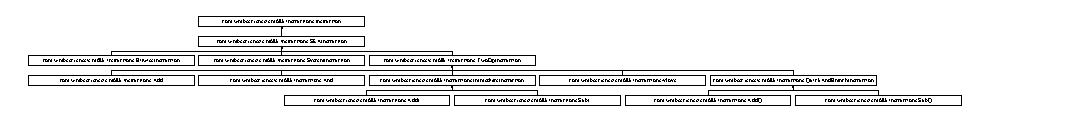
\includegraphics[height=1.193521cm]{classcom_1_1wmbest_1_1jenesis_1_1m68k_1_1instructions_1_1Instruction}
\end{center}
\end{figure}
\subsection*{Classes}
\begin{DoxyCompactItemize}
\item 
class {\bfseries Unsupported\-Opcode\-Exception}
\item 
class {\bfseries Unsupported\-Size\-Exception}
\end{DoxyCompactItemize}
\subsection*{Public Member Functions}
\begin{DoxyCompactItemize}
\item 
\hypertarget{classcom_1_1wmbest_1_1jenesis_1_1m68k_1_1instructions_1_1Instruction_a7677c16fca3ae713561735023c516619}{abstract String {\bfseries disassemble} ()}\label{classcom_1_1wmbest_1_1jenesis_1_1m68k_1_1instructions_1_1Instruction_a7677c16fca3ae713561735023c516619}

\item 
\hypertarget{classcom_1_1wmbest_1_1jenesis_1_1m68k_1_1instructions_1_1Instruction_a959e9eac7eb4f16d24289ac45b135a86}{void {\bfseries call} ()}\label{classcom_1_1wmbest_1_1jenesis_1_1m68k_1_1instructions_1_1Instruction_a959e9eac7eb4f16d24289ac45b135a86}

\item 
\hypertarget{classcom_1_1wmbest_1_1jenesis_1_1m68k_1_1instructions_1_1Instruction_ad4e0dcee77ed7094ac338d7b8aae43d6}{void {\bfseries setup} (int value)}\label{classcom_1_1wmbest_1_1jenesis_1_1m68k_1_1instructions_1_1Instruction_ad4e0dcee77ed7094ac338d7b8aae43d6}

\item 
\hypertarget{classcom_1_1wmbest_1_1jenesis_1_1m68k_1_1instructions_1_1Instruction_a9c49b686ecae04280f5c6c7e38140896}{String {\bfseries to\-String} ()}\label{classcom_1_1wmbest_1_1jenesis_1_1m68k_1_1instructions_1_1Instruction_a9c49b686ecae04280f5c6c7e38140896}

\end{DoxyCompactItemize}
\subsection*{Static Public Member Functions}
\begin{DoxyCompactItemize}
\item 
\hypertarget{classcom_1_1wmbest_1_1jenesis_1_1m68k_1_1instructions_1_1Instruction_ab5fae1036b35bcecf0affa8d5fe3e281}{static int {\bfseries size\-To\-Byte} (int size)}\label{classcom_1_1wmbest_1_1jenesis_1_1m68k_1_1instructions_1_1Instruction_ab5fae1036b35bcecf0affa8d5fe3e281}

\item 
\hypertarget{classcom_1_1wmbest_1_1jenesis_1_1m68k_1_1instructions_1_1Instruction_a04e5554f531d48dec988648d1728dd3e}{static long {\bfseries sign\-Extend} (int val, int size)}\label{classcom_1_1wmbest_1_1jenesis_1_1m68k_1_1instructions_1_1Instruction_a04e5554f531d48dec988648d1728dd3e}

\item 
\hypertarget{classcom_1_1wmbest_1_1jenesis_1_1m68k_1_1instructions_1_1Instruction_aaa9862dda2a2732431600bc52936e4b4}{static \hyperlink{classcom_1_1wmbest_1_1jenesis_1_1m68k_1_1instructions_1_1Instruction}{Instruction} {\bfseries get\-Instruction} (\hyperlink{classcom_1_1wmbest_1_1jenesis_1_1m68k_1_1SixtyEightK}{Sixty\-Eight\-K} cpu, int value)}\label{classcom_1_1wmbest_1_1jenesis_1_1m68k_1_1instructions_1_1Instruction_aaa9862dda2a2732431600bc52936e4b4}

\end{DoxyCompactItemize}
\subsection*{Public Attributes}
\begin{DoxyCompactItemize}
\item 
\hypertarget{classcom_1_1wmbest_1_1jenesis_1_1m68k_1_1instructions_1_1Instruction_a0f1791c6a76024814fffd1819f1ccdd7}{\hyperlink{classcom_1_1wmbest_1_1jenesis_1_1m68k_1_1SixtyEightK}{Sixty\-Eight\-K} {\bfseries cpu}}\label{classcom_1_1wmbest_1_1jenesis_1_1m68k_1_1instructions_1_1Instruction_a0f1791c6a76024814fffd1819f1ccdd7}

\item 
\hypertarget{classcom_1_1wmbest_1_1jenesis_1_1m68k_1_1instructions_1_1Instruction_af2904806552a247266b0cdae84a1692d}{int {\bfseries value}}\label{classcom_1_1wmbest_1_1jenesis_1_1m68k_1_1instructions_1_1Instruction_af2904806552a247266b0cdae84a1692d}

\item 
\hypertarget{classcom_1_1wmbest_1_1jenesis_1_1m68k_1_1instructions_1_1Instruction_a760da9ef24dd97d39c0833b56e01aea1}{int {\bfseries cost} = 1}\label{classcom_1_1wmbest_1_1jenesis_1_1m68k_1_1instructions_1_1Instruction_a760da9ef24dd97d39c0833b56e01aea1}

\item 
\hypertarget{classcom_1_1wmbest_1_1jenesis_1_1m68k_1_1instructions_1_1Instruction_aa0769663d2097c1fbdb27c801c417a80}{\hyperlink{classcom_1_1wmbest_1_1jenesis_1_1m68k_1_1Operand}{Operand}\mbox{[}$\,$\mbox{]} {\bfseries operands} = new \hyperlink{classcom_1_1wmbest_1_1jenesis_1_1m68k_1_1Operand}{Operand}\mbox{[}2\mbox{]}}\label{classcom_1_1wmbest_1_1jenesis_1_1m68k_1_1instructions_1_1Instruction_aa0769663d2097c1fbdb27c801c417a80}

\item 
\hypertarget{classcom_1_1wmbest_1_1jenesis_1_1m68k_1_1instructions_1_1Instruction_aa14b13c71138708579145fdf8d4bb6cf}{String {\bfseries name} = \char`\"{}I\-N\-V\-A\-L\-I\-D\char`\"{}}\label{classcom_1_1wmbest_1_1jenesis_1_1m68k_1_1instructions_1_1Instruction_aa14b13c71138708579145fdf8d4bb6cf}

\end{DoxyCompactItemize}
\subsection*{Static Public Attributes}
\begin{DoxyCompactItemize}
\item 
\hypertarget{classcom_1_1wmbest_1_1jenesis_1_1m68k_1_1instructions_1_1Instruction_a8881c49e1cdfab06fd0d1bd75768225d}{static final int {\bfseries B\-Y\-T\-E} = 1}\label{classcom_1_1wmbest_1_1jenesis_1_1m68k_1_1instructions_1_1Instruction_a8881c49e1cdfab06fd0d1bd75768225d}

\item 
\hypertarget{classcom_1_1wmbest_1_1jenesis_1_1m68k_1_1instructions_1_1Instruction_a097711cc1f7462c39374f07703dc460e}{static final int {\bfseries W\-O\-R\-D} = 3}\label{classcom_1_1wmbest_1_1jenesis_1_1m68k_1_1instructions_1_1Instruction_a097711cc1f7462c39374f07703dc460e}

\item 
\hypertarget{classcom_1_1wmbest_1_1jenesis_1_1m68k_1_1instructions_1_1Instruction_a801fe1a92552f4504ce9ee196533d34b}{static final int {\bfseries L\-O\-N\-G} = 2}\label{classcom_1_1wmbest_1_1jenesis_1_1m68k_1_1instructions_1_1Instruction_a801fe1a92552f4504ce9ee196533d34b}

\item 
\hypertarget{classcom_1_1wmbest_1_1jenesis_1_1m68k_1_1instructions_1_1Instruction_a75c7a424c091b6791710e3d3fb4f76e5}{static final int {\bfseries B\-\_\-\-S\-C\-A\-L\-E} = 1}\label{classcom_1_1wmbest_1_1jenesis_1_1m68k_1_1instructions_1_1Instruction_a75c7a424c091b6791710e3d3fb4f76e5}

\item 
\hypertarget{classcom_1_1wmbest_1_1jenesis_1_1m68k_1_1instructions_1_1Instruction_ad183a8d7ad9ad5aedfa491d8aa6157ff}{static final int {\bfseries W\-\_\-\-S\-C\-A\-L\-E} = 2}\label{classcom_1_1wmbest_1_1jenesis_1_1m68k_1_1instructions_1_1Instruction_ad183a8d7ad9ad5aedfa491d8aa6157ff}

\item 
\hypertarget{classcom_1_1wmbest_1_1jenesis_1_1m68k_1_1instructions_1_1Instruction_aa710c7bd1465591dd3226e3c11c9fdaf}{static final int {\bfseries L\-\_\-\-S\-C\-A\-L\-E} = 4}\label{classcom_1_1wmbest_1_1jenesis_1_1m68k_1_1instructions_1_1Instruction_aa710c7bd1465591dd3226e3c11c9fdaf}

\item 
\hypertarget{classcom_1_1wmbest_1_1jenesis_1_1m68k_1_1instructions_1_1Instruction_ac71aceb924125caa4203bcc10fd149f3}{static final String\mbox{[}$\,$\mbox{]} {\bfseries S\-I\-Z\-E\-\_\-\-S\-T\-R\-I\-N\-G} = new String\mbox{[}$\,$\mbox{]} \{\char`\"{}I\-N\-V\-A\-L\-I\-D\char`\"{}, \char`\"{}B\-Y\-T\-E\char`\"{}, \char`\"{}L\-O\-N\-G\char`\"{}, \char`\"{}W\-O\-R\-D\char`\"{}\}}\label{classcom_1_1wmbest_1_1jenesis_1_1m68k_1_1instructions_1_1Instruction_ac71aceb924125caa4203bcc10fd149f3}

\end{DoxyCompactItemize}
\subsection*{Protected Member Functions}
\begin{DoxyCompactItemize}
\item 
\hypertarget{classcom_1_1wmbest_1_1jenesis_1_1m68k_1_1instructions_1_1Instruction_ad65cf811ce02795e7b84db158457871b}{abstract void {\bfseries handle} ()}\label{classcom_1_1wmbest_1_1jenesis_1_1m68k_1_1instructions_1_1Instruction_ad65cf811ce02795e7b84db158457871b}

\end{DoxyCompactItemize}
\subsection*{Static Protected Member Functions}
\begin{DoxyCompactItemize}
\item 
\hypertarget{classcom_1_1wmbest_1_1jenesis_1_1m68k_1_1instructions_1_1Instruction_aa7934428325b635ba443aadce472afb2}{static boolean {\bfseries check\-Bits} (int value, int mask)}\label{classcom_1_1wmbest_1_1jenesis_1_1m68k_1_1instructions_1_1Instruction_aa7934428325b635ba443aadce472afb2}

\end{DoxyCompactItemize}


The documentation for this class was generated from the following file\-:\begin{DoxyCompactItemize}
\item 
src/main/java/com/wmbest/jenesis/m68k/instructions/Instruction.\-java\end{DoxyCompactItemize}

\hypertarget{classcom_1_1wmbest_1_1jenesis_1_1Main}{\section{com.\-wmbest.\-jenesis.\-Main Class Reference}
\label{classcom_1_1wmbest_1_1jenesis_1_1Main}\index{com.\-wmbest.\-jenesis.\-Main@{com.\-wmbest.\-jenesis.\-Main}}
}
\subsection*{Static Public Member Functions}
\begin{DoxyCompactItemize}
\item 
\hypertarget{classcom_1_1wmbest_1_1jenesis_1_1Main_abb053ca40dd2eeabb6b0307911ecb75c}{static void {\bfseries main} (String\mbox{[}$\,$\mbox{]} args)}\label{classcom_1_1wmbest_1_1jenesis_1_1Main_abb053ca40dd2eeabb6b0307911ecb75c}

\end{DoxyCompactItemize}


The documentation for this class was generated from the following file\-:\begin{DoxyCompactItemize}
\item 
src/main/java/com/wmbest/jenesis/Main.\-java\end{DoxyCompactItemize}

\hypertarget{classcom_1_1wmbest_1_1jenesis_1_1memory_1_1Memory}{\section{com.\-wmbest.\-jenesis.\-memory.\-Memory Class Reference}
\label{classcom_1_1wmbest_1_1jenesis_1_1memory_1_1Memory}\index{com.\-wmbest.\-jenesis.\-memory.\-Memory@{com.\-wmbest.\-jenesis.\-memory.\-Memory}}
}
\subsection*{Public Member Functions}
\begin{DoxyCompactItemize}
\item 
\hypertarget{classcom_1_1wmbest_1_1jenesis_1_1memory_1_1Memory_a03517687ad6ede32242b0ae486285abb}{int {\bfseries get} (int index)}\label{classcom_1_1wmbest_1_1jenesis_1_1memory_1_1Memory_a03517687ad6ede32242b0ae486285abb}

\item 
\hypertarget{classcom_1_1wmbest_1_1jenesis_1_1memory_1_1Memory_a04f913a9a838c3c92a9e7859b8232c27}{void {\bfseries set} (int index, int val)}\label{classcom_1_1wmbest_1_1jenesis_1_1memory_1_1Memory_a04f913a9a838c3c92a9e7859b8232c27}

\item 
\hypertarget{classcom_1_1wmbest_1_1jenesis_1_1memory_1_1Memory_a56c68b03edfb58f89d29fcf56fa0577c}{void {\bfseries put} (int val)}\label{classcom_1_1wmbest_1_1jenesis_1_1memory_1_1Memory_a56c68b03edfb58f89d29fcf56fa0577c}

\item 
\hypertarget{classcom_1_1wmbest_1_1jenesis_1_1memory_1_1Memory_a06351f245ecde5e30dc0afbef6293634}{void {\bfseries clear} ()}\label{classcom_1_1wmbest_1_1jenesis_1_1memory_1_1Memory_a06351f245ecde5e30dc0afbef6293634}

\end{DoxyCompactItemize}
\subsection*{Static Public Attributes}
\begin{DoxyCompactItemize}
\item 
\hypertarget{classcom_1_1wmbest_1_1jenesis_1_1memory_1_1Memory_ac89ea0e719c15a7186197d3b61ee2f56}{static Byte\-Buffer {\bfseries buffer} = Byte\-Buffer.\-allocate(0xffffff)}\label{classcom_1_1wmbest_1_1jenesis_1_1memory_1_1Memory_ac89ea0e719c15a7186197d3b61ee2f56}

\end{DoxyCompactItemize}


The documentation for this class was generated from the following file\-:\begin{DoxyCompactItemize}
\item 
src/main/java/com/wmbest/jenesis/memory/Memory.\-java\end{DoxyCompactItemize}

\hypertarget{classcom_1_1wmbest_1_1jenesis_1_1m68k_1_1instructions_1_1Move}{\section{com.\-wmbest.\-jenesis.\-m68k.\-instructions.\-Move Class Reference}
\label{classcom_1_1wmbest_1_1jenesis_1_1m68k_1_1instructions_1_1Move}\index{com.\-wmbest.\-jenesis.\-m68k.\-instructions.\-Move@{com.\-wmbest.\-jenesis.\-m68k.\-instructions.\-Move}}
}
Inheritance diagram for com.\-wmbest.\-jenesis.\-m68k.\-instructions.\-Move\-:\begin{figure}[H]
\begin{center}
\leavevmode
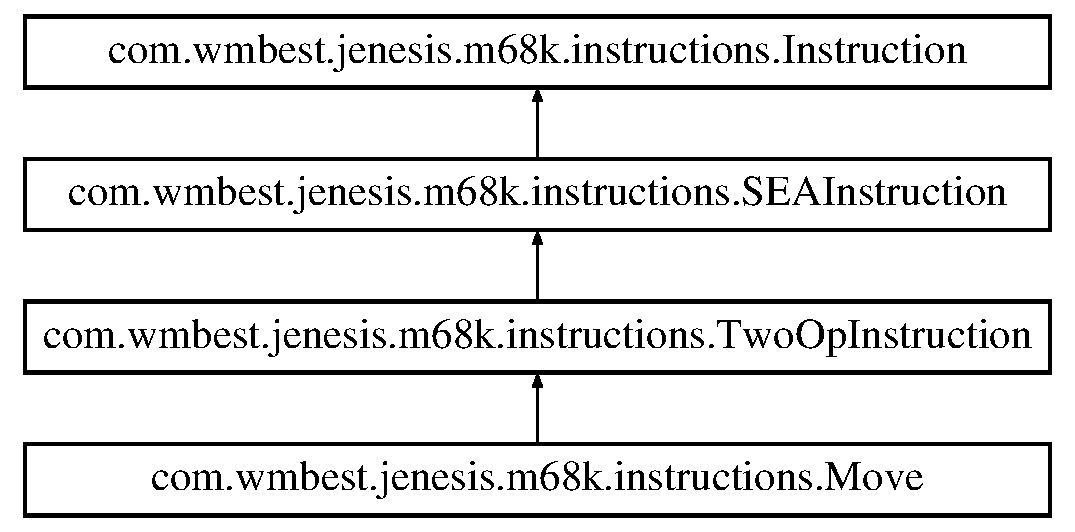
\includegraphics[height=4.000000cm]{classcom_1_1wmbest_1_1jenesis_1_1m68k_1_1instructions_1_1Move}
\end{center}
\end{figure}
\subsection*{Public Member Functions}
\begin{DoxyCompactItemize}
\item 
\hypertarget{classcom_1_1wmbest_1_1jenesis_1_1m68k_1_1instructions_1_1Move_a9ae55dd5389636bd5b22dd052c577410}{void {\bfseries setup} (int value)}\label{classcom_1_1wmbest_1_1jenesis_1_1m68k_1_1instructions_1_1Move_a9ae55dd5389636bd5b22dd052c577410}

\item 
\hypertarget{classcom_1_1wmbest_1_1jenesis_1_1m68k_1_1instructions_1_1Move_aeb72e6d56d0fd5a581c0aea951e6bb49}{void {\bfseries handle} ()}\label{classcom_1_1wmbest_1_1jenesis_1_1m68k_1_1instructions_1_1Move_aeb72e6d56d0fd5a581c0aea951e6bb49}

\item 
\hypertarget{classcom_1_1wmbest_1_1jenesis_1_1m68k_1_1instructions_1_1Move_a6b084bbdafeac7fcea4a9664c406b2e4}{String {\bfseries disassemble} ()}\label{classcom_1_1wmbest_1_1jenesis_1_1m68k_1_1instructions_1_1Move_a6b084bbdafeac7fcea4a9664c406b2e4}

\end{DoxyCompactItemize}
\subsection*{Additional Inherited Members}


The documentation for this class was generated from the following file\-:\begin{DoxyCompactItemize}
\item 
src/main/java/com/wmbest/jenesis/m68k/instructions/Move.\-java\end{DoxyCompactItemize}

\hypertarget{classcom_1_1wmbest_1_1jenesis_1_1m68k_1_1Operand}{\section{com.\-wmbest.\-jenesis.\-m68k.\-Operand Class Reference}
\label{classcom_1_1wmbest_1_1jenesis_1_1m68k_1_1Operand}\index{com.\-wmbest.\-jenesis.\-m68k.\-Operand@{com.\-wmbest.\-jenesis.\-m68k.\-Operand}}
}
\subsection*{Classes}
\begin{DoxyCompactItemize}
\item 
class {\bfseries Unsupported\-Operand\-Exception}
\end{DoxyCompactItemize}
\subsection*{Public Member Functions}
\begin{DoxyCompactItemize}
\item 
\hypertarget{classcom_1_1wmbest_1_1jenesis_1_1m68k_1_1Operand_a285ab3caa88f6610f6195e95a3f1883d}{void {\bfseries pre\-Handle} ()}\label{classcom_1_1wmbest_1_1jenesis_1_1m68k_1_1Operand_a285ab3caa88f6610f6195e95a3f1883d}

\item 
\hypertarget{classcom_1_1wmbest_1_1jenesis_1_1m68k_1_1Operand_af361d2a9715cff0bca4d337c84edfb73}{void {\bfseries post\-Handle} ()}\label{classcom_1_1wmbest_1_1jenesis_1_1m68k_1_1Operand_af361d2a9715cff0bca4d337c84edfb73}

\item 
\hypertarget{classcom_1_1wmbest_1_1jenesis_1_1m68k_1_1Operand_a9e2d1bb6f551ab8575f7b372055f5d6a}{long {\bfseries get\-Val} ()}\label{classcom_1_1wmbest_1_1jenesis_1_1m68k_1_1Operand_a9e2d1bb6f551ab8575f7b372055f5d6a}

\item 
void \hyperlink{classcom_1_1wmbest_1_1jenesis_1_1m68k_1_1Operand_a0216c18d36ae0ec59bd4e9b79294856f}{set\-Val} (long val)
\item 
\hypertarget{classcom_1_1wmbest_1_1jenesis_1_1m68k_1_1Operand_a6016e1d1e0fe49aa60f11079f9c9c843}{int {\bfseries immediate\-Byte} ()}\label{classcom_1_1wmbest_1_1jenesis_1_1m68k_1_1Operand_a6016e1d1e0fe49aa60f11079f9c9c843}

\item 
\hypertarget{classcom_1_1wmbest_1_1jenesis_1_1m68k_1_1Operand_aea77952ab2c06574d3db19a0576d26b6}{int {\bfseries immediate\-Word} ()}\label{classcom_1_1wmbest_1_1jenesis_1_1m68k_1_1Operand_aea77952ab2c06574d3db19a0576d26b6}

\item 
\hypertarget{classcom_1_1wmbest_1_1jenesis_1_1m68k_1_1Operand_ae9aebb863d2e7408e894d7bca065912b}{long {\bfseries immediate\-Long} ()}\label{classcom_1_1wmbest_1_1jenesis_1_1m68k_1_1Operand_ae9aebb863d2e7408e894d7bca065912b}

\end{DoxyCompactItemize}
\subsection*{Public Attributes}
\begin{DoxyCompactItemize}
\item 
\hypertarget{classcom_1_1wmbest_1_1jenesis_1_1m68k_1_1Operand_a1eb3049da7b9bbf9c25e3e1157a022d7}{int {\bfseries mode}}\label{classcom_1_1wmbest_1_1jenesis_1_1m68k_1_1Operand_a1eb3049da7b9bbf9c25e3e1157a022d7}

\item 
\hypertarget{classcom_1_1wmbest_1_1jenesis_1_1m68k_1_1Operand_a447d0a056ee3174d294b00cf795d3062}{int {\bfseries reg}}\label{classcom_1_1wmbest_1_1jenesis_1_1m68k_1_1Operand_a447d0a056ee3174d294b00cf795d3062}

\item 
\hypertarget{classcom_1_1wmbest_1_1jenesis_1_1m68k_1_1Operand_ab14a20d22d13ea6c3fc6448ace7a5dc0}{int {\bfseries size}}\label{classcom_1_1wmbest_1_1jenesis_1_1m68k_1_1Operand_ab14a20d22d13ea6c3fc6448ace7a5dc0}

\item 
\hypertarget{classcom_1_1wmbest_1_1jenesis_1_1m68k_1_1Operand_ac7ec6820ed9f34881ff060e055b8b162}{\hyperlink{classcom_1_1wmbest_1_1jenesis_1_1m68k_1_1SixtyEightK}{Sixty\-Eight\-K} {\bfseries cpu}}\label{classcom_1_1wmbest_1_1jenesis_1_1m68k_1_1Operand_ac7ec6820ed9f34881ff060e055b8b162}

\item 
\hypertarget{classcom_1_1wmbest_1_1jenesis_1_1m68k_1_1Operand_a44e5d7843c02bdabda73f235aad33e77}{int {\bfseries upper\-Word}}\label{classcom_1_1wmbest_1_1jenesis_1_1m68k_1_1Operand_a44e5d7843c02bdabda73f235aad33e77}

\item 
\hypertarget{classcom_1_1wmbest_1_1jenesis_1_1m68k_1_1Operand_af2f10fddcd332ef64a73341ea9935586}{int {\bfseries lower\-Word}}\label{classcom_1_1wmbest_1_1jenesis_1_1m68k_1_1Operand_af2f10fddcd332ef64a73341ea9935586}

\end{DoxyCompactItemize}


\subsection{Member Function Documentation}
\hypertarget{classcom_1_1wmbest_1_1jenesis_1_1m68k_1_1Operand_a0216c18d36ae0ec59bd4e9b79294856f}{\index{com\-::wmbest\-::jenesis\-::m68k\-::\-Operand@{com\-::wmbest\-::jenesis\-::m68k\-::\-Operand}!set\-Val@{set\-Val}}
\index{set\-Val@{set\-Val}!com::wmbest::jenesis::m68k::Operand@{com\-::wmbest\-::jenesis\-::m68k\-::\-Operand}}
\subsubsection[{set\-Val}]{\setlength{\rightskip}{0pt plus 5cm}void com.\-wmbest.\-jenesis.\-m68k.\-Operand.\-set\-Val (
\begin{DoxyParamCaption}
\item[{long}]{val}
\end{DoxyParamCaption}
)}}\label{classcom_1_1wmbest_1_1jenesis_1_1m68k_1_1Operand_a0216c18d36ae0ec59bd4e9b79294856f}
$<$ Indirect Pre\-Increment... see \hyperlink{}{pre\-Handle()}

$<$ Indirect Post\-Increment... see \hyperlink{}{post\-Handle()} 

The documentation for this class was generated from the following file\-:\begin{DoxyCompactItemize}
\item 
src/main/java/com/wmbest/jenesis/m68k/Operand.\-java\end{DoxyCompactItemize}

\hypertarget{classcom_1_1wmbest_1_1jenesis_1_1m68k_1_1instructions_1_1QuickAndBranchInstruction}{\section{com.\-wmbest.\-jenesis.\-m68k.\-instructions.\-Quick\-And\-Branch\-Instruction Class Reference}
\label{classcom_1_1wmbest_1_1jenesis_1_1m68k_1_1instructions_1_1QuickAndBranchInstruction}\index{com.\-wmbest.\-jenesis.\-m68k.\-instructions.\-Quick\-And\-Branch\-Instruction@{com.\-wmbest.\-jenesis.\-m68k.\-instructions.\-Quick\-And\-Branch\-Instruction}}
}
Inheritance diagram for com.\-wmbest.\-jenesis.\-m68k.\-instructions.\-Quick\-And\-Branch\-Instruction\-:\begin{figure}[H]
\begin{center}
\leavevmode
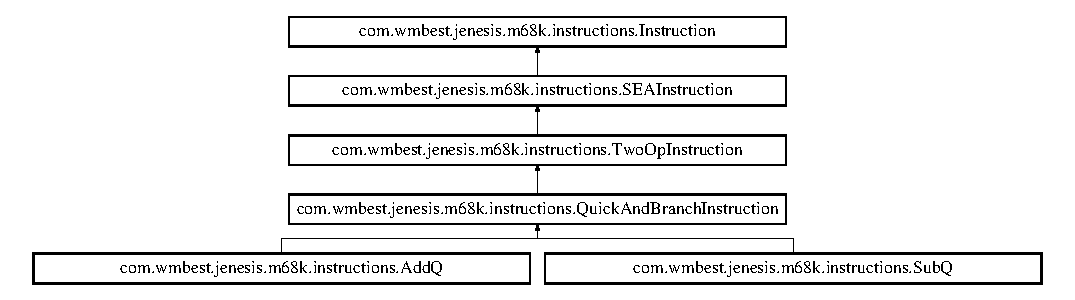
\includegraphics[height=3.580563cm]{classcom_1_1wmbest_1_1jenesis_1_1m68k_1_1instructions_1_1QuickAndBranchInstruction}
\end{center}
\end{figure}
\subsection*{Static Public Member Functions}
\begin{DoxyCompactItemize}
\item 
static \hyperlink{classcom_1_1wmbest_1_1jenesis_1_1m68k_1_1instructions_1_1QuickAndBranchInstruction}{Quick\-And\-Branch\-Instruction} \hyperlink{classcom_1_1wmbest_1_1jenesis_1_1m68k_1_1instructions_1_1QuickAndBranchInstruction_a926e056f81d08cc66c893fcce53bce6a}{get\-Instruction} (int value)
\end{DoxyCompactItemize}
\subsection*{Additional Inherited Members}


\subsection{Member Function Documentation}
\hypertarget{classcom_1_1wmbest_1_1jenesis_1_1m68k_1_1instructions_1_1QuickAndBranchInstruction_a926e056f81d08cc66c893fcce53bce6a}{\index{com\-::wmbest\-::jenesis\-::m68k\-::instructions\-::\-Quick\-And\-Branch\-Instruction@{com\-::wmbest\-::jenesis\-::m68k\-::instructions\-::\-Quick\-And\-Branch\-Instruction}!get\-Instruction@{get\-Instruction}}
\index{get\-Instruction@{get\-Instruction}!com::wmbest::jenesis::m68k::instructions::QuickAndBranchInstruction@{com\-::wmbest\-::jenesis\-::m68k\-::instructions\-::\-Quick\-And\-Branch\-Instruction}}
\subsubsection[{get\-Instruction}]{\setlength{\rightskip}{0pt plus 5cm}static {\bf Quick\-And\-Branch\-Instruction} com.\-wmbest.\-jenesis.\-m68k.\-instructions.\-Quick\-And\-Branch\-Instruction.\-get\-Instruction (
\begin{DoxyParamCaption}
\item[{int}]{value}
\end{DoxyParamCaption}
)\hspace{0.3cm}{\ttfamily [static]}}}\label{classcom_1_1wmbest_1_1jenesis_1_1m68k_1_1instructions_1_1QuickAndBranchInstruction_a926e056f81d08cc66c893fcce53bce6a}
\begin{DoxyRefDesc}{Todo}
\item[\hyperlink{todo__todo000016}{Todo}]D\-Bcc \end{DoxyRefDesc}


\begin{DoxyRefDesc}{Todo}
\item[\hyperlink{todo__todo000017}{Todo}]Scc \end{DoxyRefDesc}


\begin{DoxyRefDesc}{Todo}
\item[\hyperlink{todo__todo000018}{Todo}]B\-R\-A \end{DoxyRefDesc}


\begin{DoxyRefDesc}{Todo}
\item[\hyperlink{todo__todo000019}{Todo}]B\-S\-R \end{DoxyRefDesc}


\begin{DoxyRefDesc}{Todo}
\item[\hyperlink{todo__todo000020}{Todo}]Bcc \end{DoxyRefDesc}


\begin{DoxyRefDesc}{Todo}
\item[\hyperlink{todo__todo000021}{Todo}]M\-O\-V\-E\-Q \end{DoxyRefDesc}


The documentation for this class was generated from the following file\-:\begin{DoxyCompactItemize}
\item 
src/main/java/com/wmbest/jenesis/m68k/instructions/Quick\-And\-Branch\-Instruction.\-java\end{DoxyCompactItemize}

\hypertarget{classcom_1_1wmbest_1_1jenesis_1_1rom_1_1Rom}{\section{com.\-wmbest.\-jenesis.\-rom.\-Rom Class Reference}
\label{classcom_1_1wmbest_1_1jenesis_1_1rom_1_1Rom}\index{com.\-wmbest.\-jenesis.\-rom.\-Rom@{com.\-wmbest.\-jenesis.\-rom.\-Rom}}
}
Inheritance diagram for com.\-wmbest.\-jenesis.\-rom.\-Rom\-:\begin{figure}[H]
\begin{center}
\leavevmode
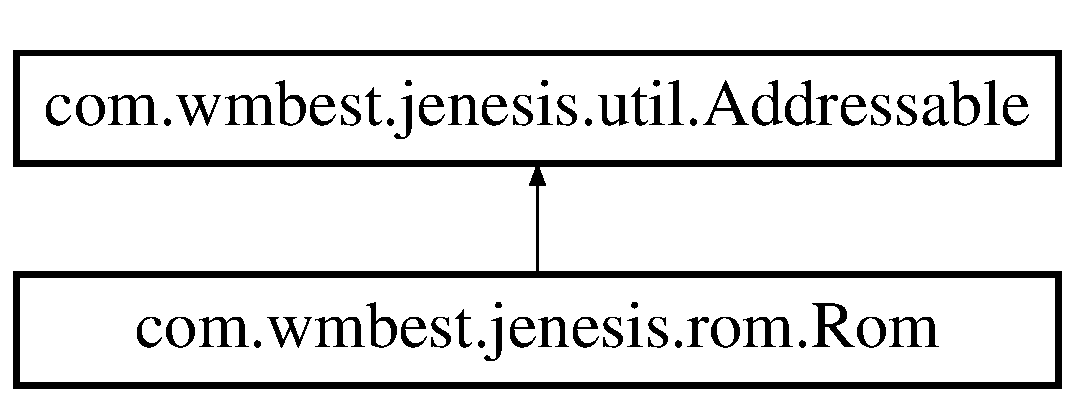
\includegraphics[height=2.000000cm]{classcom_1_1wmbest_1_1jenesis_1_1rom_1_1Rom}
\end{center}
\end{figure}
\subsection*{Public Member Functions}
\begin{DoxyCompactItemize}
\item 
\hypertarget{classcom_1_1wmbest_1_1jenesis_1_1rom_1_1Rom_ac4504ad0bc5ece06b52348044da74dcd}{abstract \hyperlink{classcom_1_1wmbest_1_1jenesis_1_1rom_1_1Rom}{Rom} {\bfseries from\-File} ()}\label{classcom_1_1wmbest_1_1jenesis_1_1rom_1_1Rom_ac4504ad0bc5ece06b52348044da74dcd}

\item 
\hypertarget{classcom_1_1wmbest_1_1jenesis_1_1rom_1_1Rom_aa0783ed551e41f5cb9c90f6f6dadab7c}{int {\bfseries get} (int index)}\label{classcom_1_1wmbest_1_1jenesis_1_1rom_1_1Rom_aa0783ed551e41f5cb9c90f6f6dadab7c}

\item 
\hypertarget{classcom_1_1wmbest_1_1jenesis_1_1rom_1_1Rom_ac802040635ca6ba864e308e96b325c97}{void {\bfseries set} (int index, int value)}\label{classcom_1_1wmbest_1_1jenesis_1_1rom_1_1Rom_ac802040635ca6ba864e308e96b325c97}

\item 
\hypertarget{classcom_1_1wmbest_1_1jenesis_1_1rom_1_1Rom_a8c043d9cc1047c0b984aba640c9f2b46}{int {\bfseries size} ()}\label{classcom_1_1wmbest_1_1jenesis_1_1rom_1_1Rom_a8c043d9cc1047c0b984aba640c9f2b46}

\end{DoxyCompactItemize}


The documentation for this class was generated from the following file\-:\begin{DoxyCompactItemize}
\item 
src/main/java/com/wmbest/jenesis/rom/Rom.\-java\end{DoxyCompactItemize}

\hypertarget{classcom_1_1wmbest_1_1jenesis_1_1m68k_1_1instructions_1_1SEAInstruction}{\section{com.\-wmbest.\-jenesis.\-m68k.\-instructions.\-S\-E\-A\-Instruction Class Reference}
\label{classcom_1_1wmbest_1_1jenesis_1_1m68k_1_1instructions_1_1SEAInstruction}\index{com.\-wmbest.\-jenesis.\-m68k.\-instructions.\-S\-E\-A\-Instruction@{com.\-wmbest.\-jenesis.\-m68k.\-instructions.\-S\-E\-A\-Instruction}}
}
Inheritance diagram for com.\-wmbest.\-jenesis.\-m68k.\-instructions.\-S\-E\-A\-Instruction\-:\begin{figure}[H]
\begin{center}
\leavevmode
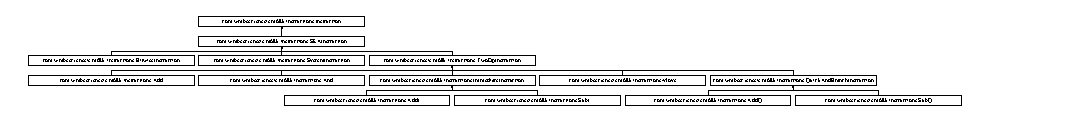
\includegraphics[height=1.193521cm]{classcom_1_1wmbest_1_1jenesis_1_1m68k_1_1instructions_1_1SEAInstruction}
\end{center}
\end{figure}
\subsection*{Public Member Functions}
\begin{DoxyCompactItemize}
\item 
\hypertarget{classcom_1_1wmbest_1_1jenesis_1_1m68k_1_1instructions_1_1SEAInstruction_a083be146ca24b617f7df57d4fcb164e0}{void {\bfseries setup} (int value)}\label{classcom_1_1wmbest_1_1jenesis_1_1m68k_1_1instructions_1_1SEAInstruction_a083be146ca24b617f7df57d4fcb164e0}

\item 
\hypertarget{classcom_1_1wmbest_1_1jenesis_1_1m68k_1_1instructions_1_1SEAInstruction_a99d9a70ba29ab5a97d40a33722690666}{int {\bfseries get\-Effective\-Register} ()}\label{classcom_1_1wmbest_1_1jenesis_1_1m68k_1_1instructions_1_1SEAInstruction_a99d9a70ba29ab5a97d40a33722690666}

\item 
\hypertarget{classcom_1_1wmbest_1_1jenesis_1_1m68k_1_1instructions_1_1SEAInstruction_acd424643d8af8a03341e4384e2231f1f}{int {\bfseries get\-Effective\-Mode} ()}\label{classcom_1_1wmbest_1_1jenesis_1_1m68k_1_1instructions_1_1SEAInstruction_acd424643d8af8a03341e4384e2231f1f}

\item 
\hypertarget{classcom_1_1wmbest_1_1jenesis_1_1m68k_1_1instructions_1_1SEAInstruction_ae448e9cdfc952938e31c8980b02a1a7a}{int {\bfseries get\-Register} (int val)}\label{classcom_1_1wmbest_1_1jenesis_1_1m68k_1_1instructions_1_1SEAInstruction_ae448e9cdfc952938e31c8980b02a1a7a}

\item 
\hypertarget{classcom_1_1wmbest_1_1jenesis_1_1m68k_1_1instructions_1_1SEAInstruction_ae14a25d50bf96fbd815aa1aedd72a798}{int {\bfseries get\-Mode} (int val)}\label{classcom_1_1wmbest_1_1jenesis_1_1m68k_1_1instructions_1_1SEAInstruction_ae14a25d50bf96fbd815aa1aedd72a798}

\item 
\hypertarget{classcom_1_1wmbest_1_1jenesis_1_1m68k_1_1instructions_1_1SEAInstruction_a64180546217f85fd8e54a54dc7097e39}{String {\bfseries to\-String} ()}\label{classcom_1_1wmbest_1_1jenesis_1_1m68k_1_1instructions_1_1SEAInstruction_a64180546217f85fd8e54a54dc7097e39}

\end{DoxyCompactItemize}
\subsection*{Static Public Attributes}
\begin{DoxyCompactItemize}
\item 
\hypertarget{classcom_1_1wmbest_1_1jenesis_1_1m68k_1_1instructions_1_1SEAInstruction_ad369b8db0254823f299199a3371d6d59}{static final int {\bfseries A\-D\-D\-R\-E\-S\-S\-\_\-\-M\-A\-S\-K} = 0x7}\label{classcom_1_1wmbest_1_1jenesis_1_1m68k_1_1instructions_1_1SEAInstruction_ad369b8db0254823f299199a3371d6d59}

\item 
\hypertarget{classcom_1_1wmbest_1_1jenesis_1_1m68k_1_1instructions_1_1SEAInstruction_aadf883dfbf4cf8e0f68161616cfb33e2}{static final int {\bfseries M\-O\-D\-E\-\_\-\-S\-H\-I\-F\-T} = 3}\label{classcom_1_1wmbest_1_1jenesis_1_1m68k_1_1instructions_1_1SEAInstruction_aadf883dfbf4cf8e0f68161616cfb33e2}

\item 
\hypertarget{classcom_1_1wmbest_1_1jenesis_1_1m68k_1_1instructions_1_1SEAInstruction_ac76dc03f73e6ed7eb027b4a58f178ac4}{static final int {\bfseries O\-P\-\_\-\-S\-H\-I\-F\-T} = 6}\label{classcom_1_1wmbest_1_1jenesis_1_1m68k_1_1instructions_1_1SEAInstruction_ac76dc03f73e6ed7eb027b4a58f178ac4}

\end{DoxyCompactItemize}
\subsection*{Additional Inherited Members}


\subsection{Detailed Description}
Most common \hyperlink{classcom_1_1wmbest_1_1jenesis_1_1m68k_1_1instructions_1_1Instruction}{Instruction} type

Defines basic behavior for Single Effective Address Instructions

See \href{http://emu-docs.org/CPU%2068k/68kpm.pdf}{\tt http\-://emu-\/docs.\-org/\-C\-P\-U\%2068k/68kpm.\-pdf} section 2-\/1 

The documentation for this class was generated from the following file\-:\begin{DoxyCompactItemize}
\item 
src/main/java/com/wmbest/jenesis/m68k/instructions/S\-E\-A\-Instruction.\-java\end{DoxyCompactItemize}

\hypertarget{classcom_1_1wmbest_1_1jenesis_1_1m68k_1_1SixtyEightK}{\section{com.\-wmbest.\-jenesis.\-m68k.\-Sixty\-Eight\-K Class Reference}
\label{classcom_1_1wmbest_1_1jenesis_1_1m68k_1_1SixtyEightK}\index{com.\-wmbest.\-jenesis.\-m68k.\-Sixty\-Eight\-K@{com.\-wmbest.\-jenesis.\-m68k.\-Sixty\-Eight\-K}}
}
\subsection*{Public Member Functions}
\begin{DoxyCompactItemize}
\item 
\hypertarget{classcom_1_1wmbest_1_1jenesis_1_1m68k_1_1SixtyEightK_add05e45fa7dc652958fac67a0a3604e7}{{\bfseries Sixty\-Eight\-K} (Memory a\-Mem)}\label{classcom_1_1wmbest_1_1jenesis_1_1m68k_1_1SixtyEightK_add05e45fa7dc652958fac67a0a3604e7}

\item 
\hypertarget{classcom_1_1wmbest_1_1jenesis_1_1m68k_1_1SixtyEightK_abe829ff42d3f776f7decdcad57f27360}{void {\bfseries run} ()}\label{classcom_1_1wmbest_1_1jenesis_1_1m68k_1_1SixtyEightK_abe829ff42d3f776f7decdcad57f27360}

\item 
\hypertarget{classcom_1_1wmbest_1_1jenesis_1_1m68k_1_1SixtyEightK_a4246faf1c578e6296966b3f54df9ca78}{void {\bfseries tick} ()}\label{classcom_1_1wmbest_1_1jenesis_1_1m68k_1_1SixtyEightK_a4246faf1c578e6296966b3f54df9ca78}

\item 
\hypertarget{classcom_1_1wmbest_1_1jenesis_1_1m68k_1_1SixtyEightK_a1ab0c1e96f4e59c799526611bddbabb3}{long {\bfseries get\-P\-C} ()}\label{classcom_1_1wmbest_1_1jenesis_1_1m68k_1_1SixtyEightK_a1ab0c1e96f4e59c799526611bddbabb3}

\item 
\hypertarget{classcom_1_1wmbest_1_1jenesis_1_1m68k_1_1SixtyEightK_a19627bfd505b0af5085c90c6ce1a8263}{long {\bfseries incr\-P\-C} ()}\label{classcom_1_1wmbest_1_1jenesis_1_1m68k_1_1SixtyEightK_a19627bfd505b0af5085c90c6ce1a8263}

\item 
\hypertarget{classcom_1_1wmbest_1_1jenesis_1_1m68k_1_1SixtyEightK_a819bf47bf9c23e41f8c83f248e37e3ae}{void {\bfseries set\-P\-C} (long a\-P\-C)}\label{classcom_1_1wmbest_1_1jenesis_1_1m68k_1_1SixtyEightK_a819bf47bf9c23e41f8c83f248e37e3ae}

\item 
\hypertarget{classcom_1_1wmbest_1_1jenesis_1_1m68k_1_1SixtyEightK_a886f9f96e004e91a7ac98529a721fed1}{long {\bfseries get\-Dx} (long x)}\label{classcom_1_1wmbest_1_1jenesis_1_1m68k_1_1SixtyEightK_a886f9f96e004e91a7ac98529a721fed1}

\item 
\hypertarget{classcom_1_1wmbest_1_1jenesis_1_1m68k_1_1SixtyEightK_ada7a0942fb9cbefdfea43ed90c0a1915}{void {\bfseries set\-Dx} (long x, long val)}\label{classcom_1_1wmbest_1_1jenesis_1_1m68k_1_1SixtyEightK_ada7a0942fb9cbefdfea43ed90c0a1915}

\item 
\hypertarget{classcom_1_1wmbest_1_1jenesis_1_1m68k_1_1SixtyEightK_a847d01a84c97e084a875eb563ab4b6af}{long {\bfseries get\-Ax} (long x)}\label{classcom_1_1wmbest_1_1jenesis_1_1m68k_1_1SixtyEightK_a847d01a84c97e084a875eb563ab4b6af}

\item 
\hypertarget{classcom_1_1wmbest_1_1jenesis_1_1m68k_1_1SixtyEightK_a1fd28011015e980bb65b96fb3549c00b}{void {\bfseries set\-Ax} (long x, long val)}\label{classcom_1_1wmbest_1_1jenesis_1_1m68k_1_1SixtyEightK_a1fd28011015e980bb65b96fb3549c00b}

\item 
\hypertarget{classcom_1_1wmbest_1_1jenesis_1_1m68k_1_1SixtyEightK_a3e06ae2ae19d3e1d6616ffec30832006}{int {\bfseries ccr} ()}\label{classcom_1_1wmbest_1_1jenesis_1_1m68k_1_1SixtyEightK_a3e06ae2ae19d3e1d6616ffec30832006}

\item 
\hypertarget{classcom_1_1wmbest_1_1jenesis_1_1m68k_1_1SixtyEightK_acbc013eeb19901e312513cca00ca25c9}{int {\bfseries get\-X\-Bit} ()}\label{classcom_1_1wmbest_1_1jenesis_1_1m68k_1_1SixtyEightK_acbc013eeb19901e312513cca00ca25c9}

\item 
\hypertarget{classcom_1_1wmbest_1_1jenesis_1_1m68k_1_1SixtyEightK_aa088884ab02683b301e892dfa3d6832b}{String {\bfseries to\-String} ()}\label{classcom_1_1wmbest_1_1jenesis_1_1m68k_1_1SixtyEightK_aa088884ab02683b301e892dfa3d6832b}

\end{DoxyCompactItemize}
\subsection*{Public Attributes}
\begin{DoxyCompactItemize}
\item 
\hypertarget{classcom_1_1wmbest_1_1jenesis_1_1m68k_1_1SixtyEightK_a67ad24f8ae64a9f9972b23614f0a159d}{Memory {\bfseries memory}}\label{classcom_1_1wmbest_1_1jenesis_1_1m68k_1_1SixtyEightK_a67ad24f8ae64a9f9972b23614f0a159d}

\end{DoxyCompactItemize}
\subsection*{Static Public Attributes}
\begin{DoxyCompactItemize}
\item 
\hypertarget{classcom_1_1wmbest_1_1jenesis_1_1m68k_1_1SixtyEightK_a89d165fb486aa40724eecbd1656ea305}{static final int {\bfseries B\-Y\-T\-E\-\_\-\-M\-A\-S\-K} = 0x000000ff}\label{classcom_1_1wmbest_1_1jenesis_1_1m68k_1_1SixtyEightK_a89d165fb486aa40724eecbd1656ea305}

\item 
\hypertarget{classcom_1_1wmbest_1_1jenesis_1_1m68k_1_1SixtyEightK_ad980f1bebdcbdd0a01382b8aa35d418c}{static final int {\bfseries N\-O\-T\-\_\-\-B\-Y\-T\-E\-\_\-\-M\-A\-S\-K} = 0xffffff00}\label{classcom_1_1wmbest_1_1jenesis_1_1m68k_1_1SixtyEightK_ad980f1bebdcbdd0a01382b8aa35d418c}

\item 
\hypertarget{classcom_1_1wmbest_1_1jenesis_1_1m68k_1_1SixtyEightK_a5f872548a9957c354376d879f140f0ff}{static final int {\bfseries W\-O\-R\-D\-\_\-\-M\-A\-S\-K} = 0x0000ffff}\label{classcom_1_1wmbest_1_1jenesis_1_1m68k_1_1SixtyEightK_a5f872548a9957c354376d879f140f0ff}

\item 
\hypertarget{classcom_1_1wmbest_1_1jenesis_1_1m68k_1_1SixtyEightK_a676b6196f43aa796d5d20fcced1bb797}{static final int {\bfseries N\-O\-T\-\_\-\-W\-O\-R\-D\-\_\-\-M\-A\-S\-K} = 0xffff0000}\label{classcom_1_1wmbest_1_1jenesis_1_1m68k_1_1SixtyEightK_a676b6196f43aa796d5d20fcced1bb797}

\end{DoxyCompactItemize}


The documentation for this class was generated from the following file\-:\begin{DoxyCompactItemize}
\item 
src/main/java/com/wmbest/jenesis/m68k/Sixty\-Eight\-K.\-java\end{DoxyCompactItemize}

\hypertarget{classcom_1_1wmbest_1_1jenesis_1_1m68k_1_1instructions_1_1SubI}{\section{com.\-wmbest.\-jenesis.\-m68k.\-instructions.\-Sub\-I Class Reference}
\label{classcom_1_1wmbest_1_1jenesis_1_1m68k_1_1instructions_1_1SubI}\index{com.\-wmbest.\-jenesis.\-m68k.\-instructions.\-Sub\-I@{com.\-wmbest.\-jenesis.\-m68k.\-instructions.\-Sub\-I}}
}
Inheritance diagram for com.\-wmbest.\-jenesis.\-m68k.\-instructions.\-Sub\-I\-:\begin{figure}[H]
\begin{center}
\leavevmode
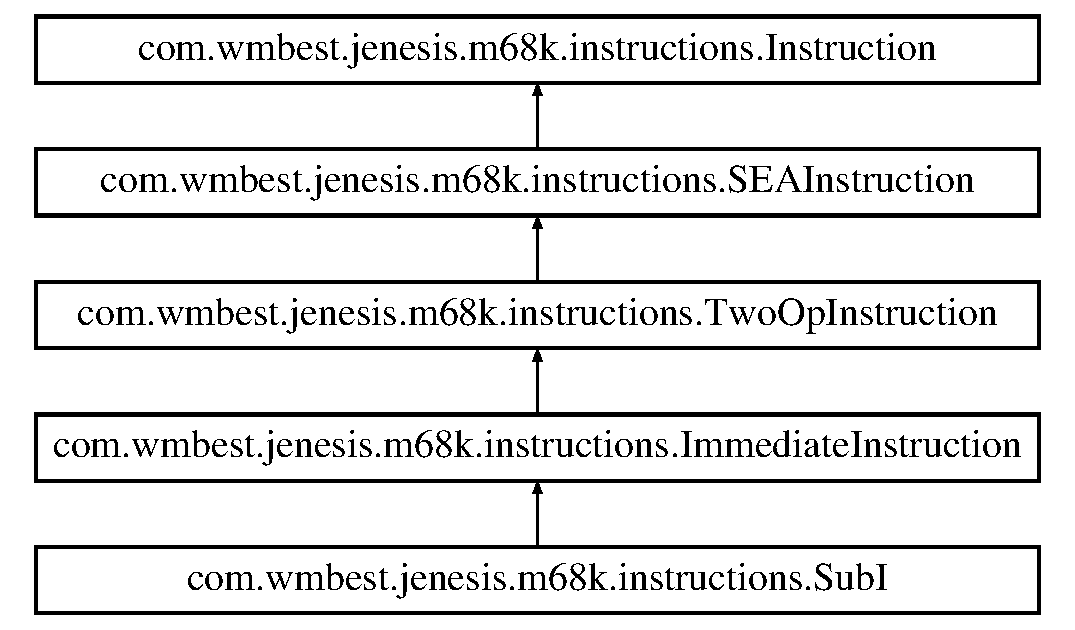
\includegraphics[height=5.000000cm]{classcom_1_1wmbest_1_1jenesis_1_1m68k_1_1instructions_1_1SubI}
\end{center}
\end{figure}
\subsection*{Public Member Functions}
\begin{DoxyCompactItemize}
\item 
\hypertarget{classcom_1_1wmbest_1_1jenesis_1_1m68k_1_1instructions_1_1SubI_a3829cd067af96dc98b5d3a25a62ee5d8}{void {\bfseries setup} (int value)}\label{classcom_1_1wmbest_1_1jenesis_1_1m68k_1_1instructions_1_1SubI_a3829cd067af96dc98b5d3a25a62ee5d8}

\item 
\hypertarget{classcom_1_1wmbest_1_1jenesis_1_1m68k_1_1instructions_1_1SubI_afffd587b5bc8c58d3e78bbc889d359be}{void {\bfseries handle} ()}\label{classcom_1_1wmbest_1_1jenesis_1_1m68k_1_1instructions_1_1SubI_afffd587b5bc8c58d3e78bbc889d359be}

\item 
\hypertarget{classcom_1_1wmbest_1_1jenesis_1_1m68k_1_1instructions_1_1SubI_ad9049b3efd1457ba6527554fbf87be32}{String {\bfseries disassemble} ()}\label{classcom_1_1wmbest_1_1jenesis_1_1m68k_1_1instructions_1_1SubI_ad9049b3efd1457ba6527554fbf87be32}

\end{DoxyCompactItemize}
\subsection*{Additional Inherited Members}


The documentation for this class was generated from the following file\-:\begin{DoxyCompactItemize}
\item 
src/main/java/com/wmbest/jenesis/m68k/instructions/Sub\-I.\-java\end{DoxyCompactItemize}

\hypertarget{classcom_1_1wmbest_1_1jenesis_1_1m68k_1_1instructions_1_1SubQ}{\section{com.\-wmbest.\-jenesis.\-m68k.\-instructions.\-Sub\-Q Class Reference}
\label{classcom_1_1wmbest_1_1jenesis_1_1m68k_1_1instructions_1_1SubQ}\index{com.\-wmbest.\-jenesis.\-m68k.\-instructions.\-Sub\-Q@{com.\-wmbest.\-jenesis.\-m68k.\-instructions.\-Sub\-Q}}
}
Inheritance diagram for com.\-wmbest.\-jenesis.\-m68k.\-instructions.\-Sub\-Q\-:\begin{figure}[H]
\begin{center}
\leavevmode
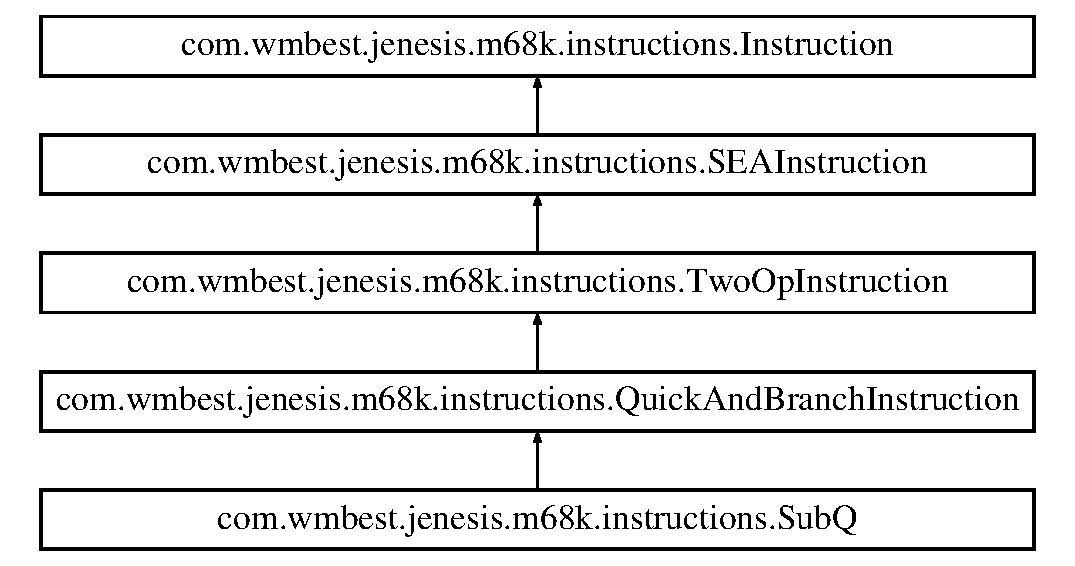
\includegraphics[height=5.000000cm]{classcom_1_1wmbest_1_1jenesis_1_1m68k_1_1instructions_1_1SubQ}
\end{center}
\end{figure}
\subsection*{Public Member Functions}
\begin{DoxyCompactItemize}
\item 
\hypertarget{classcom_1_1wmbest_1_1jenesis_1_1m68k_1_1instructions_1_1SubQ_ae7a84a277d0702df067c4bc311cbdc4b}{void {\bfseries setup} (int value)}\label{classcom_1_1wmbest_1_1jenesis_1_1m68k_1_1instructions_1_1SubQ_ae7a84a277d0702df067c4bc311cbdc4b}

\item 
\hypertarget{classcom_1_1wmbest_1_1jenesis_1_1m68k_1_1instructions_1_1SubQ_a558554b5d8c96f7ab60cfd87f45841bf}{void {\bfseries handle} ()}\label{classcom_1_1wmbest_1_1jenesis_1_1m68k_1_1instructions_1_1SubQ_a558554b5d8c96f7ab60cfd87f45841bf}

\item 
\hypertarget{classcom_1_1wmbest_1_1jenesis_1_1m68k_1_1instructions_1_1SubQ_af29368048c25265618e13bb58a62e23f}{String {\bfseries disassemble} ()}\label{classcom_1_1wmbest_1_1jenesis_1_1m68k_1_1instructions_1_1SubQ_af29368048c25265618e13bb58a62e23f}

\end{DoxyCompactItemize}
\subsection*{Additional Inherited Members}


The documentation for this class was generated from the following file\-:\begin{DoxyCompactItemize}
\item 
src/main/java/com/wmbest/jenesis/m68k/instructions/Sub\-Q.\-java\end{DoxyCompactItemize}

\hypertarget{classcom_1_1wmbest_1_1jenesis_1_1m68k_1_1instructions_1_1SystemInstruction}{\section{com.\-wmbest.\-jenesis.\-m68k.\-instructions.\-System\-Instruction Class Reference}
\label{classcom_1_1wmbest_1_1jenesis_1_1m68k_1_1instructions_1_1SystemInstruction}\index{com.\-wmbest.\-jenesis.\-m68k.\-instructions.\-System\-Instruction@{com.\-wmbest.\-jenesis.\-m68k.\-instructions.\-System\-Instruction}}
}
Inheritance diagram for com.\-wmbest.\-jenesis.\-m68k.\-instructions.\-System\-Instruction\-:\begin{figure}[H]
\begin{center}
\leavevmode
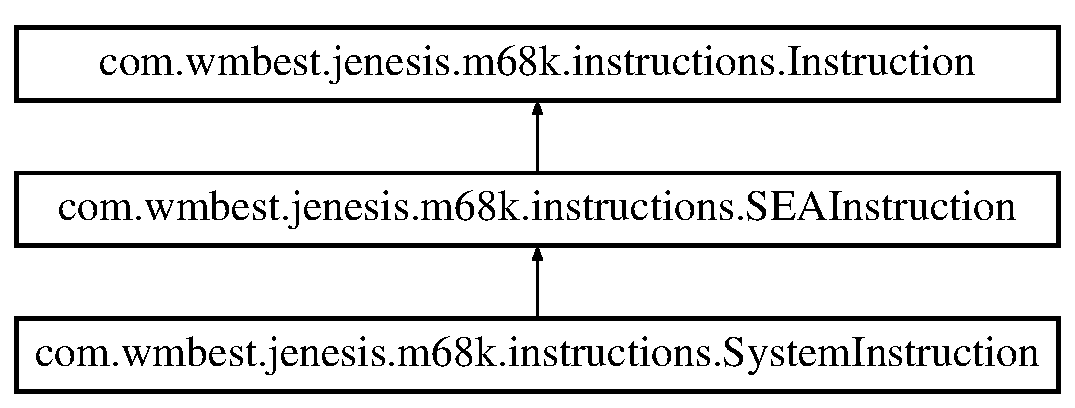
\includegraphics[height=3.000000cm]{classcom_1_1wmbest_1_1jenesis_1_1m68k_1_1instructions_1_1SystemInstruction}
\end{center}
\end{figure}
\subsection*{Static Public Member Functions}
\begin{DoxyCompactItemize}
\item 
static \hyperlink{classcom_1_1wmbest_1_1jenesis_1_1m68k_1_1instructions_1_1SystemInstruction}{System\-Instruction} \hyperlink{classcom_1_1wmbest_1_1jenesis_1_1m68k_1_1instructions_1_1SystemInstruction_a3a02281c96164bd836be2eca75873c07}{get\-Instruction} (int value)
\end{DoxyCompactItemize}
\subsection*{Additional Inherited Members}


\subsection{Member Function Documentation}
\hypertarget{classcom_1_1wmbest_1_1jenesis_1_1m68k_1_1instructions_1_1SystemInstruction_a3a02281c96164bd836be2eca75873c07}{\index{com\-::wmbest\-::jenesis\-::m68k\-::instructions\-::\-System\-Instruction@{com\-::wmbest\-::jenesis\-::m68k\-::instructions\-::\-System\-Instruction}!get\-Instruction@{get\-Instruction}}
\index{get\-Instruction@{get\-Instruction}!com::wmbest::jenesis::m68k::instructions::SystemInstruction@{com\-::wmbest\-::jenesis\-::m68k\-::instructions\-::\-System\-Instruction}}
\subsubsection[{get\-Instruction}]{\setlength{\rightskip}{0pt plus 5cm}static {\bf System\-Instruction} com.\-wmbest.\-jenesis.\-m68k.\-instructions.\-System\-Instruction.\-get\-Instruction (
\begin{DoxyParamCaption}
\item[{int}]{value}
\end{DoxyParamCaption}
)\hspace{0.3cm}{\ttfamily [static]}}}\label{classcom_1_1wmbest_1_1jenesis_1_1m68k_1_1instructions_1_1SystemInstruction_a3a02281c96164bd836be2eca75873c07}
\begin{DoxyRefDesc}{Todo}
\item[\hyperlink{todo__todo000022}{Todo}]I\-L\-L\-E\-G\-A\-L \end{DoxyRefDesc}


\begin{DoxyRefDesc}{Todo}
\item[\hyperlink{todo__todo000023}{Todo}]R\-E\-S\-E\-T \end{DoxyRefDesc}


\begin{DoxyRefDesc}{Todo}
\item[\hyperlink{todo__todo000024}{Todo}]N\-O\-P \end{DoxyRefDesc}


\begin{DoxyRefDesc}{Todo}
\item[\hyperlink{todo__todo000025}{Todo}]S\-T\-O\-P \end{DoxyRefDesc}


\begin{DoxyRefDesc}{Todo}
\item[\hyperlink{todo__todo000026}{Todo}]R\-T\-E \end{DoxyRefDesc}


\begin{DoxyRefDesc}{Todo}
\item[\hyperlink{todo__todo000027}{Todo}]R\-T\-S \end{DoxyRefDesc}


\begin{DoxyRefDesc}{Todo}
\item[\hyperlink{todo__todo000028}{Todo}]T\-R\-A\-P\-V \end{DoxyRefDesc}


\begin{DoxyRefDesc}{Todo}
\item[\hyperlink{todo__todo000029}{Todo}]R\-T\-R \end{DoxyRefDesc}


\begin{DoxyRefDesc}{Todo}
\item[\hyperlink{todo__todo000030}{Todo}]T\-R\-A\-P \end{DoxyRefDesc}


\begin{DoxyRefDesc}{Todo}
\item[\hyperlink{todo__todo000031}{Todo}]L\-I\-N\-K (ea M\-O\-D\-E 0b010) \end{DoxyRefDesc}


\begin{DoxyRefDesc}{Todo}
\item[\hyperlink{todo__todo000032}{Todo}]U\-N\-L\-K (ea M\-O\-D\-E 0b011) \end{DoxyRefDesc}


\begin{DoxyRefDesc}{Todo}
\item[\hyperlink{todo__todo000033}{Todo}]M\-O\-V\-E U\-S\-P \end{DoxyRefDesc}


\begin{DoxyRefDesc}{Todo}
\item[\hyperlink{todo__todo000034}{Todo}]M\-O\-V\-E from S\-R (size 0b11) \end{DoxyRefDesc}


\begin{DoxyRefDesc}{Todo}
\item[\hyperlink{todo__todo000035}{Todo}]N\-E\-G\-X (size 0b00 $\sim$ 0b10) \end{DoxyRefDesc}


\begin{DoxyRefDesc}{Todo}
\item[\hyperlink{todo__todo000036}{Todo}]M\-O\-V\-E to C\-C\-R (size 0b11) \end{DoxyRefDesc}


\begin{DoxyRefDesc}{Todo}
\item[\hyperlink{todo__todo000037}{Todo}]N\-E\-G (size 0b00 $\sim$ 0b10) \end{DoxyRefDesc}


\begin{DoxyRefDesc}{Todo}
\item[\hyperlink{todo__todo000038}{Todo}]M\-O\-V\-E to S\-R (size 0b11) \end{DoxyRefDesc}


\begin{DoxyRefDesc}{Todo}
\item[\hyperlink{todo__todo000039}{Todo}]N\-O\-T (size 0b00 $\sim$ 0b10) \end{DoxyRefDesc}


\begin{DoxyRefDesc}{Todo}
\item[\hyperlink{todo__todo000040}{Todo}]E\-X\-T (size 0b10 $\sim$ 0b11, ea M\-O\-D\-E 0b000) \end{DoxyRefDesc}


\begin{DoxyRefDesc}{Todo}
\item[\hyperlink{todo__todo000041}{Todo}]M\-O\-V\-E\-M (size 0b10 $\sim$ 0b11) \end{DoxyRefDesc}


\begin{DoxyRefDesc}{Todo}
\item[\hyperlink{todo__todo000042}{Todo}]N\-C\-B\-D (size 0b00) \end{DoxyRefDesc}


\begin{DoxyRefDesc}{Todo}
\item[\hyperlink{todo__todo000043}{Todo}]S\-W\-A\-P (size 0b01, ea M\-O\-D\-E 0b000) \end{DoxyRefDesc}


\begin{DoxyRefDesc}{Todo}
\item[\hyperlink{todo__todo000044}{Todo}]P\-E\-A (size 0b01) \end{DoxyRefDesc}


\begin{DoxyRefDesc}{Todo}
\item[\hyperlink{todo__todo000045}{Todo}]T\-A\-S (size 0b11) \end{DoxyRefDesc}


\begin{DoxyRefDesc}{Todo}
\item[\hyperlink{todo__todo000046}{Todo}]T\-S\-T (size 0b00 $\sim$ 0b10) \end{DoxyRefDesc}


\begin{DoxyRefDesc}{Todo}
\item[\hyperlink{todo__todo000047}{Todo}]M\-O\-V\-E\-M (size 0b10 $\sim$ 0b11) \end{DoxyRefDesc}


\begin{DoxyRefDesc}{Todo}
\item[\hyperlink{todo__todo000048}{Todo}]J\-S\-R (size 0b10) \end{DoxyRefDesc}


\begin{DoxyRefDesc}{Todo}
\item[\hyperlink{todo__todo000049}{Todo}]J\-M\-P (size 0b11) \end{DoxyRefDesc}


The documentation for this class was generated from the following file\-:\begin{DoxyCompactItemize}
\item 
src/main/java/com/wmbest/jenesis/m68k/instructions/System\-Instruction.\-java\end{DoxyCompactItemize}

\hypertarget{classcom_1_1wmbest_1_1jenesis_1_1m68k_1_1instructions_1_1TwoOpInstruction}{\section{com.\-wmbest.\-jenesis.\-m68k.\-instructions.\-Two\-Op\-Instruction Class Reference}
\label{classcom_1_1wmbest_1_1jenesis_1_1m68k_1_1instructions_1_1TwoOpInstruction}\index{com.\-wmbest.\-jenesis.\-m68k.\-instructions.\-Two\-Op\-Instruction@{com.\-wmbest.\-jenesis.\-m68k.\-instructions.\-Two\-Op\-Instruction}}
}
Inheritance diagram for com.\-wmbest.\-jenesis.\-m68k.\-instructions.\-Two\-Op\-Instruction\-:\begin{figure}[H]
\begin{center}
\leavevmode
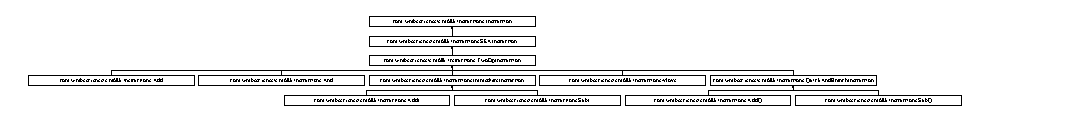
\includegraphics[height=1.193521cm]{classcom_1_1wmbest_1_1jenesis_1_1m68k_1_1instructions_1_1TwoOpInstruction}
\end{center}
\end{figure}
\subsection*{Public Member Functions}
\begin{DoxyCompactItemize}
\item 
\hypertarget{classcom_1_1wmbest_1_1jenesis_1_1m68k_1_1instructions_1_1TwoOpInstruction_a6ca82d1038853e0d8a932481dfd7d495}{void {\bfseries setup} (int value)}\label{classcom_1_1wmbest_1_1jenesis_1_1m68k_1_1instructions_1_1TwoOpInstruction_a6ca82d1038853e0d8a932481dfd7d495}

\item 
\hypertarget{classcom_1_1wmbest_1_1jenesis_1_1m68k_1_1instructions_1_1TwoOpInstruction_af2876d760d248f24d449f800519b3466}{String {\bfseries to\-String} ()}\label{classcom_1_1wmbest_1_1jenesis_1_1m68k_1_1instructions_1_1TwoOpInstruction_af2876d760d248f24d449f800519b3466}

\end{DoxyCompactItemize}
\subsection*{Additional Inherited Members}


The documentation for this class was generated from the following file\-:\begin{DoxyCompactItemize}
\item 
src/main/java/com/wmbest/jenesis/m68k/instructions/Two\-Op\-Instruction.\-java\end{DoxyCompactItemize}

\printindex
\end{document}
